% ============================================================
% MIORPA 2026 -- Research Report
% Holographic Krylov Complexity
% ============================================================
\documentclass[11pt,a4paper]{article}

% ---------- Fonts, mathematics, layout ----------
\usepackage[T1]{fontenc}
\usepackage[utf8]{inputenc}
\usepackage{lmodern}
\usepackage[a4paper,margin=1in]{geometry}
\usepackage{microtype}
\usepackage{setspace}
\onehalfspacing

\usepackage{amsmath,amssymb,amsfonts,mathtools}
\usepackage{amsthm}
\usepackage{bm}
\usepackage{physics}
\usepackage{booktabs}
\usepackage{array}
\usepackage{enumitem}
\usepackage{graphicx}
\usepackage{float}
\usepackage{xcolor}
\usepackage{tikz}
\usetikzlibrary{positioning,arrows.meta}
\usepackage{url}
\usepackage[hidelinks]{hyperref}
\usepackage[nameinlink,capitalise]{cleveref}

% ---------- Theorem environments ----------
\theoremstyle{plain}
\newtheorem{proposition}{Proposition}[section]
\newtheorem{lemma}[proposition]{Lemma}
\newtheorem{corollary}[proposition]{Corollary}

\theoremstyle{definition}
\newtheorem{definition}[proposition]{Definition}
\newtheorem{remark}[proposition]{Remark}

\theoremstyle{remark}
\newtheorem{observation}[proposition]{Numerical observation}

% ---------- Short commands ----------
\newcommand{\Routh}{\mathcal R}
\newcommand{\Krylov}{\mathcal K}
\newcommand{\Pproper}{P_{\mathrm{proper}}}
\newcommand{\PrR}{P_r^{(R)}}
\newcommand{\PetaR}{P_\eta^{(R)}}
\newcommand{\PrhoR}{P_\rho^{(R)}}
\newcommand{\Ck}{C_{\mathrm K}}
\newcommand{\meff}{m_{\mathrm{eff}}}

\newcommand{\ii}{\mathrm i}

% NOTE (repository reorganization): paths updated to match the public repository
% layout, where this .tex file lives in report/ alongside the code directories
% ads3/, quiver_comparison/, blackstring_quiver/ at the repository root. This is
% a build-path change only; no equation, figure content, or numerical value below
% was altered. See CHANGELOG.md in the repository root.
\graphicspath{{./}{../figures/}{../ads3/}{../../quiver_comparison/figures/}{../../blackstring_quiver/figures/}}

% ---------- Title ----------
\title{\textbf{Holographic Krylov Complexity}\\
\large Charged probes, fixed-charge Routhian reduction, and top-down quiver geometries}
\author{Géraud Ogounchi Badélé\\
MIORPA 2026 Participant\\
Mathematical Institute, University of Oxford}
\date{September 2026}

\begin{document}
\maketitle

\begin{abstract}
Krylov, or spread, complexity measures how a quantum state spreads along the Krylov basis generated by its Hamiltonian evolution. For a normalized state initially located at the first Krylov site, the short-time expansion is universal:
\begin{equation*}
C_{\mathrm K}(t)=b_1^2t^2+\mathcal O(t^4),\qquad
\dot C_{\mathrm K}(0)=0.
\end{equation*}
A recent holographic proposal identifies the growth rate of spread complexity with the proper radial momentum of a bulk probe. For probes carrying a conserved Noether charge, however, a naive extension that includes motion along the corresponding cyclic direction produces a non-zero initial proper momentum, apparently contradicting the quantum result. The central point of this report is that the comparison must be performed in the fixed-charge sector. A partial Legendre transform with respect to the cyclic coordinate gives a Routhian in which the cyclic degree of freedom is eliminated and its energetic effect is retained through a position-dependent effective mass. The resulting reduced radial momentum vanishes for a probe released from rest and grows linearly at short times.

We derive this mechanism for a general charged point particle, obtain a closed-form short-time coefficient in global $\mathrm{AdS}_3$, and then apply the same construction to top-down massive IIA backgrounds dual to six-dimensional $\mathcal N=(1,0)$ SCFT quivers. The reduction is tested for two distinct quiver geometries and then for a structurally different $\mathrm{AdS}_3\times S^2$ black-string-chain background with a quadratic rank-function profile. The report separates analytic consequences of Routh reduction from numerical observations and identifies the remaining limitations and natural directions for extending the analysis to genuinely extended probes.
\end{abstract}

\tableofcontents
\clearpage

% ============================================================
\section{Introduction}
\label{sec:intro}
% ============================================================

Quantum complexity provides a quantitative way of asking how difficult it becomes to represent or generate a quantum state under time evolution. Among the different notions of complexity, Krylov or spread complexity is especially useful because it is constructed directly from the dynamics generated by the Hamiltonian. Starting from an initial state, repeated action of the Hamiltonian generates a Krylov subspace, and the Lanczos algorithm produces an orthonormal basis in which the Hamiltonian takes tridiagonal form. The time-evolved state then behaves as a wavepacket on an effective one-dimensional chain \cite{Parker:2018yvk,Balasubramanian:2022tpr}.

Holography offers a complementary geometric description, built on the correspondence between quantum field theories and gravitational duals \cite{Maldacena:1997re,Gubser:1998bc,Witten:1998qj}. For heavy local excitations, a standard semiclassical dictionary replaces the boundary excitation by a massive bulk probe following a timelike geodesic. In a two-dimensional conformal field theory, Caputa et al.\ proposed a precise relation between the rate of spread complexity and the proper radial momentum of the dual probe \cite{Caputa:2024odg}. This provides a particularly simple geometric picture of state spreading: initially the state is localized near the first Krylov site, while on the gravity side the probe is released from rest and subsequently develops radial momentum.

The natural question is whether this dictionary remains consistent when the probe carries a conserved internal or angular charge. This is non-trivial. If a cyclic coordinate $\varphi$ carries a conserved Noether charge
\begin{equation*}
J=P_\varphi,
\end{equation*}
then a probe can have $\dot\varphi\neq0$ even when its radial velocity vanishes. If one naively includes this cyclic motion in a composite proper momentum, the resulting observable has a non-zero value at the initial time. Since a unitary Krylov evolution has $\dot C_{\mathrm K}(0)=0$, this produces a short-time mismatch.

The main observation developed here is that a conserved cyclic charge should be treated as a \emph{fixed sector label} before the holographic proper momentum is constructed. This is implemented by a Routhian reduction: one partially Legendre-transforms the cyclic degree of freedom and obtains a reduced Lagrangian at fixed $J$. The charge remains physically present through an effective mass or potential, but the cyclic coordinate is no longer counted as an independent direction in the radial complexity observable. This is precisely the fixed-charge prescription developed systematically for charged and extended probes in recent work \cite{Chatzis:2026ekd}.

The present report applies that idea to three settings. First, a general charged point particle is treated analytically. Second, the mechanism is made explicit in global $\mathrm{AdS}_3$, where a closed-form coefficient for the leading Krylov growth is obtained and checked numerically. Third, the same reduction is applied to top-down massive IIA geometries dual to six-dimensional SCFT quivers, first for two distinct quiver constructions and then for a quadratic-rank black-string-chain background. The purpose is not to claim a complete holographic derivation of Krylov complexity, but to isolate a precise consistency condition and test its robustness across increasingly structured geometries.

A structurally related phenomenon -- geodesic motion along a quiver coordinate that damps at a rate set by the UV cutoff, leaving a universal late-time growth -- has recently been found for top-down $\mathrm{AdS}_3$ and $\mathrm{AdS}_2$ duals of two- and one-dimensional quiver theories \cite{Fatemiabhari:2025qcg}. That analysis concerns uncharged probes and a different family of backgrounds from the six-dimensional SCFT quivers studied here, but the qualitative pattern of quiver-direction motion decoupling from a universal radial law is common to both settings.

\subsection*{Code and reproducibility}

The symbolic derivations, numerical integrations, and figure- and table-generating scripts underlying \cref{sec:ads3,sec:quivers,sec:blackstring} are publicly available at
\begin{center}
\url{https://github.com/Ogoun09gerbad/Holographic-Krylov-Complexity}
\end{center}
The repository contains the exact code used to produce every numerical figure and table in this report, together with a \texttt{REPRODUCIBILITY.md} file mapping each reported result to the script and parameters that generate it. An archived, citable release of the version corresponding to this report is deposited on Zenodo at \url{https://doi.org/REPLACE_WITH_ZENODO_DOI}; that DOI, rather than the GitHub URL, should be used for permanent citation of the code.

% ============================================================
\section{Krylov spread complexity}
\label{sec:krylov}
% ============================================================

\subsection{Quantum evolution and the Krylov subspace}

Let $\mathcal H$ be the Hilbert space of a quantum system and let
$|\psi_0\rangle\in\mathcal H$ be a normalized initial state,
\begin{equation*}
\langle\psi_0|\psi_0\rangle=1.
\end{equation*}
For a time-independent Hermitian Hamiltonian $H=H^\dagger$, the Schr\"odinger equation is
\begin{equation*}
\ii\frac{\mathrm d}{\mathrm d t}|\psi(t)\rangle
=
H|\psi(t)\rangle ,
\end{equation*}
with solution
\begin{equation*}
|\psi(t)\rangle=e^{-\ii Ht}|\psi_0\rangle .
\end{equation*}
The evolution is unitary, so the norm and therefore total probability are conserved.

The Krylov subspace generated by $H$ and $|\psi_0\rangle$ is
\begin{equation*}
\Krylov_N(H,\psi_0)
=
\operatorname{span}
\left\{
|\psi_0\rangle,
H|\psi_0\rangle,
H^2|\psi_0\rangle,\ldots,
H^{N-1}|\psi_0\rangle
\right\}.
\end{equation*}
Its infinite-dimensional version, when the chain does not terminate, will simply be denoted by $\Krylov$.

Applying the Lanczos algorithm to the sequence
$|\psi_0\rangle,H|\psi_0\rangle,\ldots$ produces an orthonormal basis
$\{|K_n\rangle\}$ satisfying
\begin{equation*}
|K_0\rangle=|\psi_0\rangle,
\end{equation*}
and
\begin{equation*}
H|K_n\rangle
=
b_{n+1}|K_{n+1}\rangle
+a_n|K_n\rangle
+b_n|K_{n-1}\rangle,
\qquad
b_0=0,
\end{equation*}
where $a_n\in\mathbb R$ and $b_n\geq0$. Thus the Hamiltonian is represented by a real symmetric tridiagonal (Jacobi) matrix in the Krylov basis.

Expanding the evolved state,
\begin{equation*}
|\psi(t)\rangle
=
\sum_{n\geq0}\phi_n(t)|K_n\rangle,
\qquad
\phi_n(t)=\langle K_n|\psi(t)\rangle,
\end{equation*}
turns the Schr\"odinger equation into a nearest-neighbour evolution on the Krylov chain,
\begin{equation*}
\ii\dot\phi_n
=
b_{n+1}\phi_{n+1}
+a_n\phi_n
+b_n\phi_{n-1}.
\end{equation*}

\begin{figure}[ht]
\centering
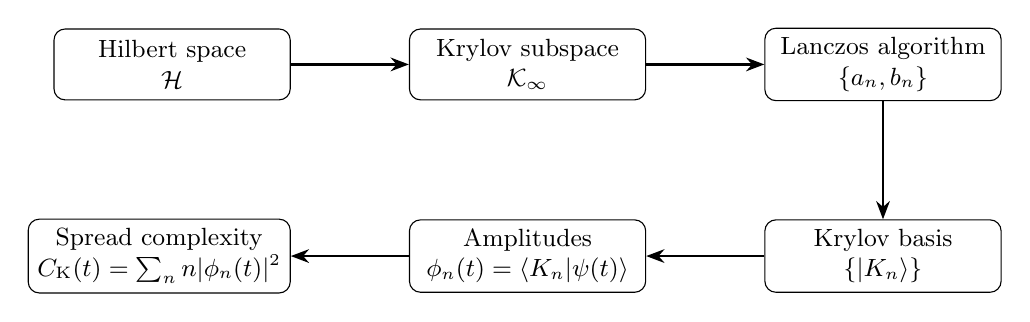
\begin{tikzpicture}[
    node distance=1.5cm,
    box/.style={
        draw,
        rounded corners,
        align=center,
        minimum width=3cm,
        minimum height=0.9cm,
        font=\small
    },
    arrow/.style={
        ->,
        >=Stealth,
        thick
    }
]
\node[box] (H)
{Hilbert space\\
$\mathcal H$};
\node[box, right=of H] (K)
{Krylov subspace\\
$\Krylov_\infty$};
\node[box, right=of K] (L)
{Lanczos algorithm\\
$\{a_n,b_n\}$};
\node[box, below=of L] (B)
{Krylov basis\\
$\{|K_n\rangle\}$};
\node[box, left=of B] (Phi)
{Amplitudes\\
$\phi_n(t)=\langle K_n|\psi(t)\rangle$};
\node[box, left=of Phi] (C)
{Spread complexity\\
$\Ck(t)=\sum_n n|\phi_n(t)|^2$};
\draw[arrow] (H) -- (K);
\draw[arrow] (K) -- (L);
\draw[arrow] (L) -- (B);
\draw[arrow] (B) -- (Phi);
\draw[arrow] (Phi) -- (C);
\end{tikzpicture}
\caption{Logical flow of the construction of Krylov complexity. Starting from a Hilbert space and an initial state, the Hamiltonian evolution generates a Krylov subspace. The Lanczos algorithm produces an orthonormal Krylov basis, whose amplitudes $\phi_n(t)$ determine the spread complexity $\Ck(t)$.}
\label{fig:flowchart}
\end{figure}

\subsection{Definition of spread complexity}

\begin{definition}[Krylov spread complexity]
The spread complexity of the state $|\psi(t)\rangle$ is
\begin{equation*}
\Ck(t)
=
\sum_{n=0}^\infty n\,|\phi_n(t)|^2.
\end{equation*}
\end{definition}

The quantity $\Ck(t)$ is the mean position of the wavepacket on the Krylov chain. The Lanczos basis is distinguished because the corresponding spread is minimal among appropriate orthonormal basis choices; this gives the construction a dynamical and basis-independent interpretation \cite{Balasubramanian:2022tpr}.

\subsection{Universal short-time behaviour}

The short-time behaviour follows directly from the Jacobi structure of the Krylov Hamiltonian.

\begin{proposition}[Evenness and initial growth]
\label{prop:evenness}
Assume $H$ is time independent and Hermitian, and choose the Lanczos basis so that the Jacobi matrix has real entries. If $|\psi(0)\rangle=|K_0\rangle$, then
\begin{equation*}
\Ck(-t)=\Ck(t),
\end{equation*}
and
\begin{equation}
\boxed{
\Ck(t)=b_1^2t^2+\mathcal O(t^4),
\qquad
\dot{\Ck}(t)=2b_1^2t+\mathcal O(t^3).
}
\label{eq:krylov-short-time}
\end{equation}
In particular,
\begin{equation*}
\boxed{\dot{\Ck}(0)=0}.
\end{equation*}
\end{proposition}

\begin{proof}
Because the Krylov Hamiltonian is real and Hermitian,
\begin{equation*}
e^{+\ii Ht}=(e^{-\ii Ht})^*.
\end{equation*}
Hence
\begin{equation*}
\phi_n(-t)=\phi_n(t)^*,
\end{equation*}
so $|\phi_n(-t)|^2=|\phi_n(t)|^2$ and therefore $\Ck(-t)=\Ck(t)$.

For the coefficient of the leading term, use
\begin{equation*}
H|K_0\rangle=a_0|K_0\rangle+b_1|K_1\rangle.
\end{equation*}
The short-time expansion gives
\begin{align*}
\phi_0(t)
&=
1-\ii a_0t
-\frac12(a_0^2+b_1^2)t^2+\mathcal O(t^3),\\
\phi_1(t)
&=
-\ii b_1t+\mathcal O(t^2),\\
\phi_{n\geq2}(t)
&=
\mathcal O(t^2).
\end{align*}
Therefore
\begin{equation*}
|\phi_1(t)|^2=b_1^2t^2+\mathcal O(t^4),
\end{equation*}
where the odd contribution cancels in the modulus squared. Contributions with $n\geq2$ start at order $t^4$. Hence
\begin{equation*}
\Ck(t)=b_1^2t^2+\mathcal O(t^4).
\end{equation*}
\end{proof}

The coefficient $b_1$ therefore provides the leading measure of the initial spreading. For the present holographic analysis, the most important consequence is not the precise value of $b_1$, but the structural condition $\dot{\Ck}(0)=0$.

As an elementary illustration, for the $3\times3$ Hamiltonian $H=\left(\begin{smallmatrix}2&1&0\\1&3&0\\0&0&4\end{smallmatrix}\right)$ acting on $|\psi_0\rangle=(1,0,0)^\top$, the Lanczos recursion terminates after two sites with $a_0=2$, $b_1=1$, $a_1=3$, $b_2=0$, so that $\Ck(t)=|\phi_1(t)|^2=t^2+\mathcal O(t^4)$ at short times; \cref{fig:toy-ct} shows the resulting $\Ck(t)$ against $t^2$.

\begin{figure}[H]
\centering
\IfFileExists{../figures/ct_example.png}
{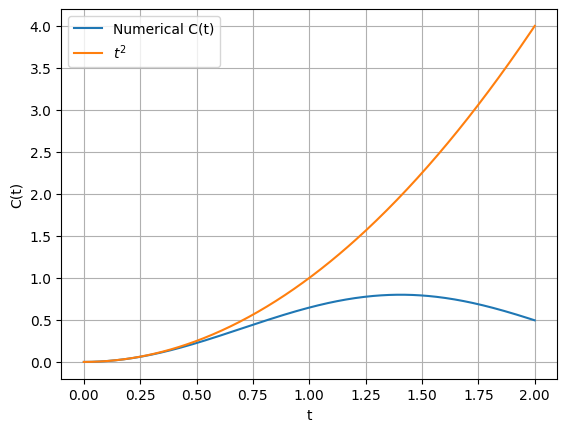
\includegraphics[width=0.5\linewidth]{ct_example.png}}
{\fbox{\parbox{0.45\linewidth}{\centering Figure to be inserted.}}}
\caption{Spread complexity $\Ck(t)$ (blue) for the $3\times3$ toy model above, compared with $t^2$ (orange). The two curves agree at short times, consistent with $C_2=b_1^2=1$; they separate once the finite Krylov chain (only two sites) is fully explored, well beyond the short-time regime that \cref{prop:evenness} controls.}
\label{fig:toy-ct}
\end{figure}

% ============================================================
\section{Holographic proper momentum and the charged-probe puzzle}
\label{sec:holo-puzzle}
% ============================================================

\subsection{Probe approximation and momentum--complexity correspondence}

The semiclassical probe approximation replaces a sufficiently heavy boundary excitation by a massive bulk particle. The bulk geometry is treated as fixed, while the probe follows a timelike worldline. The corresponding momentum--complexity proposal identifies the growth of spread complexity with a proper radial momentum,
\begin{equation}
\dot{\Ck}(t)
=
\lambda\,|\Pproper(t)|,
\qquad
\lambda>0,
\label{eq:momentum-complexity}
\end{equation}
with the overall normalization determined by the operator and by the precise holographic dictionary. This relation was made explicit for states excited by local operators in two-dimensional CFTs and global $\mathrm{AdS}_3$ probes in \cite{Caputa:2024odg}.

For a neutral probe released from rest, the proposal is naturally compatible with \cref{prop:evenness}: the radial momentum starts at zero and grows linearly at short times.

The difficulty arises when the probe has a conserved charge associated with a cyclic coordinate.

\subsection{General charged point particle}

Consider the static metric
\begin{equation*}
\mathrm d s^2
=
-f(r)\mathrm d t^2
+g(r)\mathrm d r^2
+h(r)\mathrm d\varphi^2,
\end{equation*}
and the massive point-particle Lagrangian
\begin{equation*}
L
=
-m\sqrt{
f(r)-g(r)\dot r^2-h(r)\dot\varphi^2
}.
\end{equation*}
The coordinate $\varphi$ is cyclic, hence
\begin{equation}
J
\equiv
P_\varphi
=
\frac{\partial L}{\partial\dot\varphi}
=
\frac{m h(r)\dot\varphi}
{\sqrt{f-g\dot r^2-h\dot\varphi^2}}
=
\mathrm{const}.
\label{eq:J-definition}
\end{equation}

The canonical radial momentum is
\begin{equation*}
P_r
=
\frac{\partial L}{\partial\dot r}
=
\frac{m g(r)\dot r}
{\sqrt{f-g\dot r^2-h\dot\varphi^2}}.
\end{equation*}

A natural full spatial momentum magnitude is obtained from the spatial metric,
\begin{equation}
|P_{\mathrm{full}}|
=
\sqrt{\frac{P_r^2}{g(r)}
+\frac{P_\varphi^2}{h(r)}}.
\label{eq:Pfull}
\end{equation}
At an initial radial turning point,
\begin{equation*}
\dot r(0)=0
\quad\Longrightarrow\quad
P_r(0)=0,
\end{equation*}
but
\begin{equation*}
P_\varphi(0)=J.
\end{equation*}
Consequently,
\begin{equation}
\boxed{
|P_{\mathrm{naive}}(0)|
=
\frac{|J|}{\sqrt{h(r_0)}}
\neq0
\qquad (J\neq0).
}
\label{eq:naive-intercept}
\end{equation}
If \eqref{eq:Pfull} is inserted directly into \eqref{eq:momentum-complexity}, the holographic quantity has a non-zero initial value, in conflict with \eqref{eq:krylov-short-time}.

\begin{remark}
The issue is not that the conserved charge is physically absent. The issue is that the charged cyclic motion has been included as if it were an additional direction of radial state spreading. The correct comparison should be made after reducing to the fixed-charge sector.
\end{remark}

% ============================================================
\section{Fixed-charge Routhian reduction}
\label{sec:routhian}
% ============================================================

\subsection{Partial Legendre transform}

For definiteness, this report uses the sign convention
\begin{equation}
\boxed{
R(q,\dot q;J)
=
L(q,\dot q,\dot\varphi)-J\dot\varphi,
}
\label{eq:our-routhian-convention}
\end{equation}
which is the negative of the alternative convention often used in the literature. Since this differs only by an overall sign, the Euler--Lagrange trajectories are unchanged. The important content is the partial Legendre transform at fixed $J$.

The cyclic velocity is first solved from \eqref{eq:J-definition}. One obtains
\begin{equation*}
\dot\varphi
=
\frac{
J\sqrt{f(r)-g(r)\dot r^2}
}{
\sqrt{
h(r)\left[J^2+m^2h(r)\right]
}
}.
\end{equation*}
Substitution into \eqref{eq:our-routhian-convention} gives
\begin{equation}
R(r,\dot r;J)
=
-\meff(r)
\sqrt{f(r)-g(r)\dot r^2},
\label{eq:reduced-routhian}
\end{equation}
where
\begin{equation*}
\boxed{
\meff(r)
=
\sqrt{
m^2+\frac{J^2}{h(r)}
}.
}
\end{equation*}

Thus the charge is not removed. Its dynamical effect survives through the position-dependent effective mass.

\subsection{Reduced momentum}

The reduced radial momentum is
\begin{equation}
\boxed{
\PrR
=
\frac{\partial R}{\partial\dot r}
=
\frac{
\meff(r)g(r)\dot r
}{
\sqrt{f(r)-g(r)\dot r^2}
}.
}
\label{eq:reduced-radial-momentum}
\end{equation}

\begin{lemma}[Partial Legendre transform preserves the non-cyclic momentum]
\label{lemma:routhian-momentum}
Let $q$ denote any non-cyclic coordinate. Let $\dot\varphi(q,\dot q;J)$ be obtained by solving
$J=\partial L/\partial\dot\varphi$, and define $R=L-J\dot\varphi$. Then
\begin{equation*}
\frac{\partial R}{\partial\dot q}
=
\frac{\partial L}{\partial\dot q},
\qquad
\frac{\partial R}{\partial q}
=
\frac{\partial L}{\partial q},
\end{equation*}
after the substitution $\dot\varphi=\dot\varphi(q,\dot q;J)$.
\end{lemma}

\begin{proof}
Using the chain rule,
\begin{equation*}
\frac{\partial R}{\partial\dot q}
=
\frac{\partial L}{\partial\dot q}
+
\left(
\frac{\partial L}{\partial\dot\varphi}-J
\right)
\frac{\partial\dot\varphi}{\partial\dot q}.
\end{equation*}
The quantity in parentheses vanishes identically by the defining charge constraint. Hence
\begin{equation*}
\frac{\partial R}{\partial\dot q}
=
\frac{\partial L}{\partial\dot q}.
\end{equation*}
The same calculation with $q$ in place of $\dot q$ gives the second relation.
\end{proof}

The lemma makes clear what the Routhian does and does not change. The reduced momentum is not an artificial replacement for the original radial momentum; it is the same non-cyclic canonical momentum evaluated after the cyclic degree of freedom has been eliminated at fixed charge.

\begin{corollary}[The Routhian leaves the trajectory unchanged]
\label{cor:same-trajectory}
At fixed $J$, the function $r(t)$ obtained by solving the Euler--Lagrange equation of the Routhian $R$ coincides with the function $r(t)$ obtained by solving the Euler--Lagrange equation of the original Lagrangian $L$, for the same initial data $r(0),\dot r(0)$.
\end{corollary}

\begin{proof}
By \cref{lemma:routhian-momentum} with $q=r$, $\partial R/\partial\dot r=\partial L/\partial\dot r$ and $\partial R/\partial r=\partial L/\partial r$ identically, after substituting $\dot\varphi=\dot\varphi(r,\dot r;J)$. Hence the Euler--Lagrange equation $\frac{\mathrm d}{\mathrm d t}(\partial R/\partial\dot r)=\partial R/\partial r$ is, term by term, the same differential equation for $r(t)$ as $\frac{\mathrm d}{\mathrm d t}(\partial L/\partial\dot r)=\partial L/\partial r$. Two solutions of the same second-order equation with the same initial data coincide.
\end{proof}

This clarifies precisely what changes between the naive and fixed-charge prescriptions. The probe follows one physical trajectory $r(t)$, common to both descriptions; the Routhian reduction does not alter it. What differs is only which momentum observable is read off along that trajectory: the naive prescription combines the original $P_r=\partial L/\partial\dot r$ (mass $m$) with the cyclic contribution $P_\varphi=J$ into $|P_{\mathrm{full}}|$ of \eqref{eq:Pfull}, while the fixed-charge prescription uses $\PrR=\partial R/\partial\dot r$ alone -- the same functional form as $P_r$, but with $m$ replaced by the position-dependent $\meff(r)$, and with no separate contribution from $\varphi$.

\subsection{Short-time theorem}

\begin{proposition}[Fixed-charge short-time behaviour]
\label{prop:routhian-short-time}
Suppose a probe is released at
\begin{equation*}
r(0)=r_0,
\qquad
\dot r(0)=0,
\end{equation*}
with fixed conserved charge $J$. Assume the solution is smooth. Then
\begin{equation}
\PrR(t)
=
A(J,m,r_0)t+\mathcal O(t^3),
\label{eq:Pr-short}
\end{equation}
and consequently the fixed-charge holographic prescription
\begin{equation*}
\dot{\Ck}(t)=\lambda|\PrR(t)|
\end{equation*}
gives
\begin{equation}
\dot{\Ck}(t)
=
\lambda|A|\,t+\mathcal O(t^3),
\qquad
\Ck(t)
=
\frac{\lambda|A|}{2}t^2+\mathcal O(t^4).
\label{eq:C-short-holo}
\end{equation}
\end{proposition}

\begin{proof}
The initial condition gives
\begin{equation*}
\PrR(0)=0
\end{equation*}
directly from \eqref{eq:reduced-radial-momentum}. Smoothness of the trajectory gives
\begin{equation*}
r(t)=r_0+\frac12a t^2+\mathcal O(t^4),
\qquad
\dot r(t)=at+\mathcal O(t^3),
\end{equation*}
where $a=\ddot r(0)$. Inserting this expansion into \eqref{eq:reduced-radial-momentum} produces \eqref{eq:Pr-short} for some coefficient $A$. The proposed relation \eqref{eq:momentum-complexity} then gives the first equation in \eqref{eq:C-short-holo}, and integration with $\Ck(0)=0$ gives the second.
\end{proof}

The quantum and holographic short-time structures therefore agree:
\begin{equation*}
\boxed{
\dot{\Ck}(0)=0,
\qquad
\dot{\Ck}(t)\sim t,
\qquad
\Ck(t)\sim t^2.
}
\end{equation*}

\subsection{Illustrative schematics}

The following two schematics summarize, qualitatively, the geometric picture behind \cref{prop:routhian-short-time} and the puzzle it resolves.

\begin{figure}[ht]
\centering
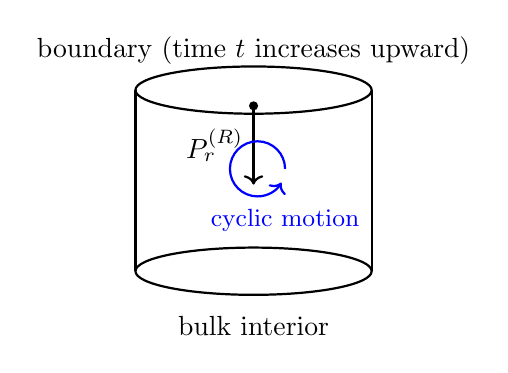
\begin{tikzpicture}[scale=1]
  \draw[thick] (0,-0.3) ellipse (1.5 and 0.3);
  \draw[thick] (-1.5,-0.3) -- (-1.5,2.0);
  \draw[thick] (1.5,-0.3) -- (1.5,2.0);
  \draw[thick] (0,2.0) ellipse (1.5 and 0.3);
  \filldraw[black] (0,1.8) circle (0.05);
  \draw[->, thick] (0,1.8) -- (0,0.8) node[midway,left] {$\PrR$};
  \draw[->, blue, thick] (0.4,1.0) arc (0:330:0.35);
  \node[blue, font=\small] at (0.4,0.35) {cyclic motion};
  \node at (0,2.5) {boundary (time $t$ increases upward)};
  \node at (0,-1.0) {bulk interior};
\end{tikzpicture}
\caption{Schematic of a bulk spacetime (cylinder) with a probe (black dot) released from rest and falling inward. The reduced radial momentum $\PrR$ vanishes at $t=0$ and grows as the probe falls; the blue arrow indicates the cyclic motion at fixed charge $J$, which is eliminated from the reduced configuration space by the Routhian but remains present through $\meff$.}
\label{fig:ads-cylinder}
\end{figure}

\begin{figure}[ht]
\centering
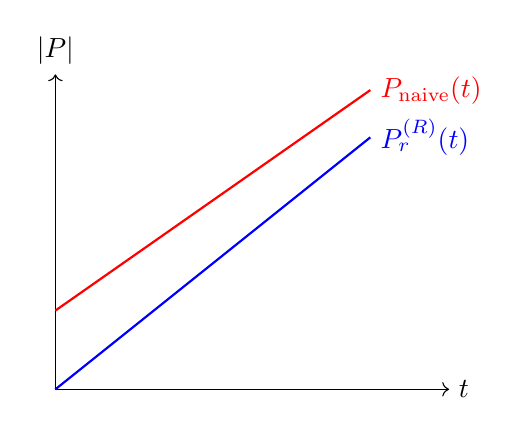
\begin{tikzpicture}[scale=1]
  \draw[->] (0,0) -- (5,0) node[right] {$t$};
  \draw[->] (0,0) -- (0,4) node[above] {$|P|$};
  \draw[blue, thick] (0,0) -- (4,3.2) node[right,blue] {$\PrR(t)$};
  \draw[red, thick] (0,1) -- (4,3.8) node[right,red] {$P_{\mathrm{naive}}(t)$};
\end{tikzpicture}
\caption{Schematic comparison of the two momentum prescriptions. The naive momentum (red) has a nonzero intercept at $t=0$ from the fixed charge $J$, cf.\ \eqref{eq:naive-intercept}; the Routhian-reduced momentum (blue) starts at zero and grows linearly, as required by $\dot{\Ck}(t)\sim t$.}
\label{fig:naive-vs-routhian-schematic}
\end{figure}

% ============================================================
\section{\texorpdfstring{Global $\mathrm{AdS}_3$}{Global AdS3}: analytic benchmark}
\label{sec:ads3}
% ============================================================

\subsection{Geometry}

The simplest concrete background is global $\mathrm{AdS}_3$, with AdS radius set to one:
\begin{equation*}
\mathrm d s^2
=
-(1+r^2)\mathrm d t^2
+
\frac{\mathrm d r^2}{1+r^2}
+
r^2\mathrm d\varphi^2 .
\end{equation*}
Thus
\begin{equation*}
f(r)=1+r^2,
\qquad
g(r)=\frac1{1+r^2},
\qquad
h(r)=r^2.
\end{equation*}

The Routhian is
\begin{equation}
R
=
-\sqrt{
m^2+\frac{J^2}{r^2}
}
\sqrt{
(1+r^2)-\frac{\dot r^2}{1+r^2}
}.
\label{eq:ads3-routhian}
\end{equation}

The conserved energy associated with time-translation invariance is
\begin{equation}
E
=
\dot r\,\frac{\partial R}{\partial\dot r}-R
=
\frac{
\meff(r)(1+r^2)
}{
\sqrt{(1+r^2)-\dot r^2/(1+r^2)}
}.
\label{eq:ads3-energy}
\end{equation}
At release from rest at $r=r_0$,
\begin{equation}
E^2
=
\left(m^2+\frac{J^2}{r_0^2}\right)(1+r_0^2).
\label{eq:ads3-energy-initial}
\end{equation}

\subsection{Initial acceleration}

It is useful to write the radial equation in first-order form,
\begin{equation}
\dot r^2
=
(1+r^2)^2
\left[
1-\frac{
\left(m^2+\frac{J^2}{r^2}\right)(1+r^2)
}{E^2}
\right].
\label{eq:ads3-radial-firstorder}
\end{equation}
With the turning-point initial condition \eqref{eq:ads3-energy-initial}, differentiating \eqref{eq:ads3-radial-firstorder} once more with respect to $t$ and evaluating at $\dot r=0$, $r=r_0$ gives the initial radial acceleration
\begin{equation*}
\boxed{
\ddot r(0)
=
\frac{
(1+r_0^2)(J^2-m^2r_0^4)
}{
r_0(m^2r_0^2+J^2)
}.
}
\end{equation*}
For the near-boundary regime $r_0\gg1$ with fixed $m$ and $J$, the $m^2r_0^4$ term dominates, so the initial acceleration is inward.

\subsection{Linear coefficient of the reduced momentum}

Expanding the reduced momentum around $t=0$ yields
\begin{equation*}
\PrR(t)
=
\alpha(J,m,r_0)\,t+\mathcal O(t^3),
\end{equation*}
with
\begin{equation}
\boxed{
\alpha(J,m,r_0)
=
\frac{
J^2-m^2r_0^4
}{
r_0^2
\sqrt{
(m^2r_0^2+J^2)(1+r_0^2)
}
}.
}
\label{eq:ads3-alpha}
\end{equation}

Combining this with the momentum--complexity proposal gives the leading holographic coefficient
\begin{equation*}
\boxed{
C_2^{\mathrm{holo}}
=
\frac{\lambda}{2}
\frac{
|J^2-m^2r_0^4|
}{
r_0^2
\sqrt{
(m^2r_0^2+J^2)(1+r_0^2)
}
}.
}
\end{equation*}

The result is manifestly non-negative, as required for $C_2=b_1^2$.

\subsection{Consistency limits}

In the neutral limit $J\to0$,
\begin{equation*}
C_2^{\mathrm{holo}}
\longrightarrow
\frac{\lambda}{2}
\frac{mr_0}{\sqrt{1+r_0^2}},
\end{equation*}
and therefore
\begin{equation*}
\lim_{r_0\to\infty}\lim_{J\to0}
C_2^{\mathrm{holo}}
=
\frac{\lambda m}{2}.
\end{equation*}

The $J\to0$ limit is an important check because the reduced and unreduced descriptions coincide when the cyclic motion is absent.

\subsection{Exact neutral trajectory in proper time}
\label{sec:ads3-exact-neutral}

The results above are short-time expansions in the coordinate time $t$. For the neutral case $J=0$ the full nonlinear radial motion can in fact be solved in closed form, giving an independent, non-perturbative cross-check that goes beyond the short-time regime.

Let $\tau$ denote proper time along the worldline, defined by $\mathrm d\tau^2\equiv-\mathrm ds^2$, and write $r'\equiv\mathrm dr/\mathrm d\tau$ (reserving $\dot r$ for $\mathrm dr/\mathrm dt$ as elsewhere in this report). Because $J=0$ implies $\meff=m$, \cref{cor:same-trajectory} guarantees that the trajectory and the conserved energy of the reduced problem coincide with those of the original, unreduced geodesic problem; in particular the constant $E$ of \eqref{eq:ads3-energy}--\eqref{eq:ads3-energy-initial} is also the Noether charge associated with the time-translation symmetry of the $\tau$-parametrized problem, $E=mf(r)\,\mathrm dt/\mathrm d\tau$. The timelike normalization $-f(\mathrm dt/\mathrm d\tau)^2+f^{-1}r'^2=-1$, together with $J=0$, then gives the proper-time radial equation
\begin{equation}
r'^2=\frac{E^2}{m^2}-1-r^2.
\label{eq:ads3-proper-time-eq}
\end{equation}

\begin{proposition}[Exact neutral trajectory]
\label{prop:ads3-exact-neutral}
A neutral probe ($J=0$) released from rest at $r=r_0$ follows, for all proper times, the exact trajectory
\begin{equation}
\boxed{
r(\tau)=r_0\cos(\tau-\tau_0),
}
\label{eq:ads3-exact-neutral}
\end{equation}
for a constant $\tau_0$ fixed by the initial condition, with $r_0$ related to $E$ exactly as in \eqref{eq:ads3-energy-initial} at $J=0$, i.e.\ $E^2=m^2(1+r_0^2)$.
\end{proposition}

\begin{proof}
By \eqref{eq:ads3-energy-initial} at $J=0$, $E^2/m^2-1=r_0^2$, so \eqref{eq:ads3-proper-time-eq} reads $r'^2=r_0^2-r^2$. Differentiating once more in $\tau$ gives $r''=-r$, the equation of a simple harmonic oscillator, with general solution $r(\tau)=r_0\cos(\tau-\tau_0)$ for the amplitude fixed by $r(\tau_0)=r_0$; substituting back verifies $r'^2=r_0^2\sin^2(\tau-\tau_0)=r_0^2-r^2$ directly, confirming \eqref{eq:ads3-proper-time-eq}.
\end{proof}

Two features of \eqref{eq:ads3-exact-neutral} are worth noting. First, it is an exact solution of the full nonlinear equation of motion, not merely a leading-order approximation; expanding \eqref{eq:ads3-exact-neutral} around $\tau=\tau_0$ reproduces the short-time behaviour of \cref{sec:ads3} order by order once $\tau$ is itself re-expanded in $t$. Second, the radial coordinate returns to the turning value $r_0$ with period $\pi$ in proper time, independently of $r_0$ (equivalently, of $E$ and $m$): this is a direct manifestation of the confining structure of $\mathrm{AdS}_3$ noted in \cref{sec:ads3} -- unlike a free particle in flat space, a massive neutral probe in global $\mathrm{AdS}_3$ can never escape to the boundary, and instead falls back on a proper-time scale set purely by the AdS radius, independent of its energy.

\subsection{Numerical validation}

Equations \eqref{eq:ads3-energy-initial}--\eqref{eq:ads3-alpha} were independently re-derived with a computer algebra system directly from the Routhian \eqref{eq:ads3-routhian}, without reference to the closed forms quoted above, and found to agree with them identically. The Euler--Lagrange equation of the same Routhian was then integrated numerically with an eighth-order adaptive Runge--Kutta method (\texttt{DOP853}, relative and absolute tolerances of order $10^{-13}$) for five representative values of $(m,J,r_0)$, including the neutral case $J=0$. The short-time slope of $\PrR(t)$ was extracted from a least-squares fit through the origin on the window $t\in[10^{-6},2\times10^{-4}]$ and compared with the closed-form coefficient $\alpha(J,m,r_0)$ of \eqref{eq:ads3-alpha}; the relative deviation was at most $1.0\times10^{-7}$ over the tested cases, consistent with the accumulated truncation and floating-point error of the integrator rather than with any discrepancy in the analytic formula. The verification script (\texttt{ads3\_validation.py}) is included with the project files and regenerates \cref{fig:ads3-validation} from these same computations.

This check confirms internal consistency between the closed-form derivation and its numerical integration for the tested parameter values; it is a code- and algebra-consistency check, not an independent test of the momentum--complexity proposal \eqref{eq:momentum-complexity} itself.

\begin{figure}[H]
\centering
\IfFileExists{../ads3/holographic_krylov_validation.png}
{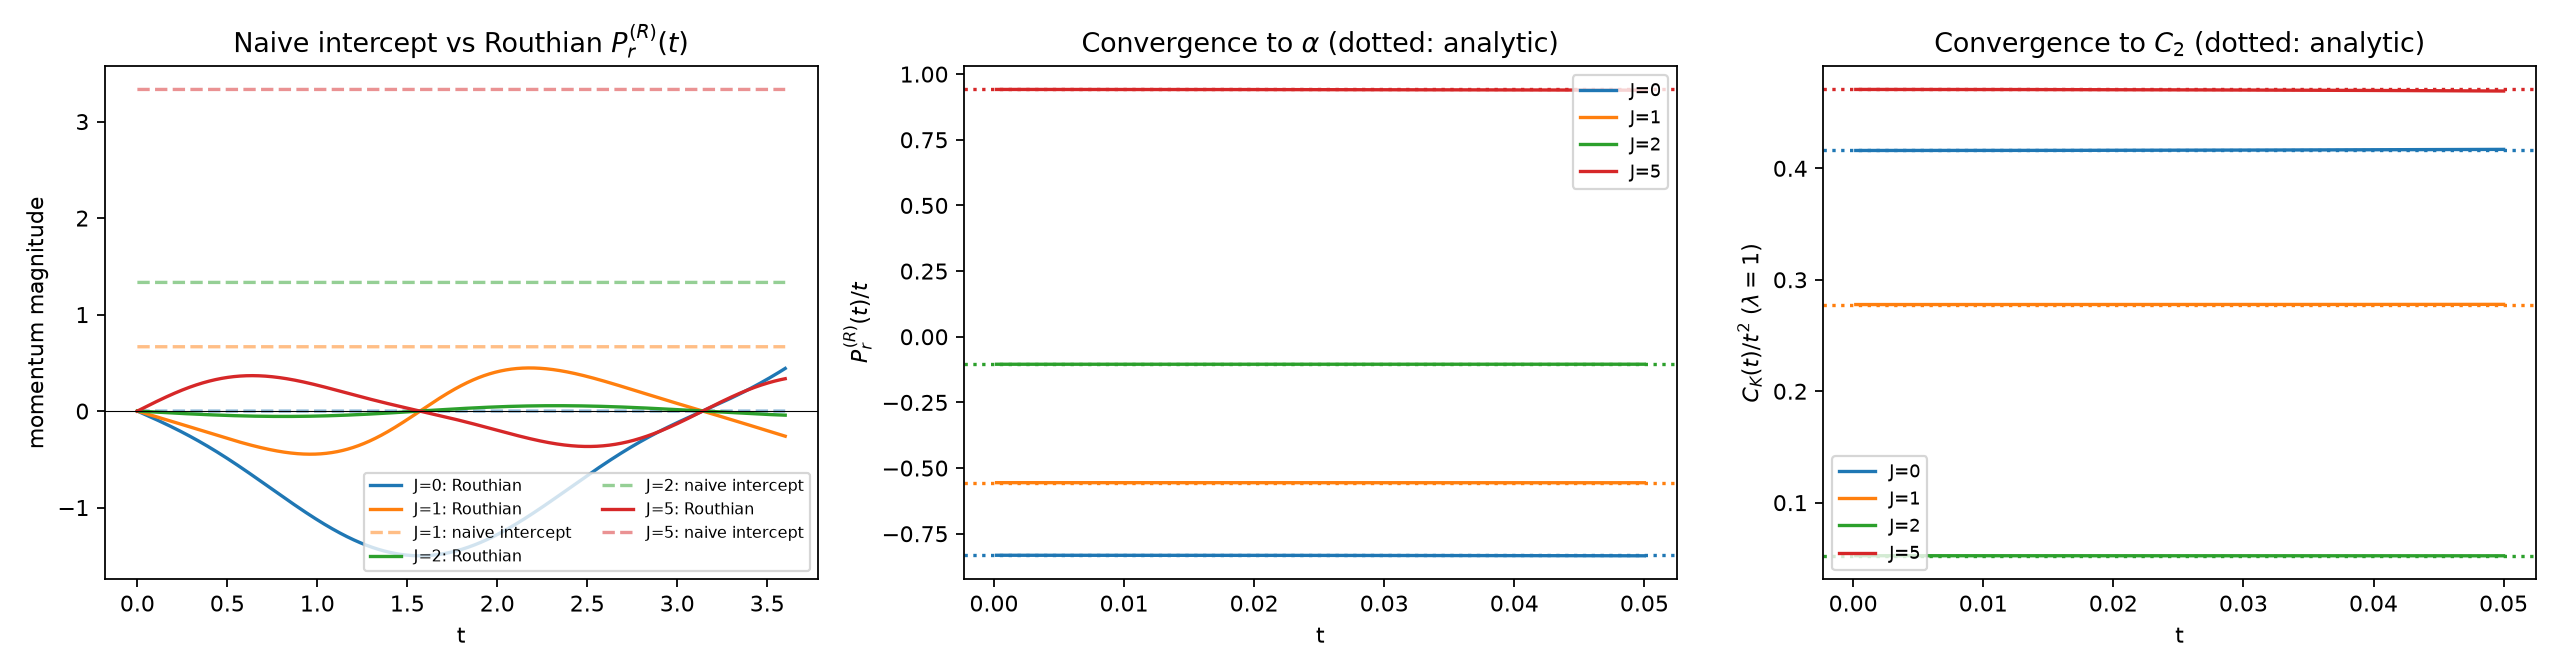
\includegraphics[width=0.72\linewidth]{holographic_krylov_validation.png}}
{\fbox{\parbox{0.7\linewidth}{\centering Numerical validation figure to be inserted from the project computation.}}}
\caption{Numerical validation in the global $\mathrm{AdS}_3$ benchmark, for $m=1$, $r_0=1.5$, and four values of $J$. \emph{Left:} the naive momentum \eqref{eq:naive-intercept} is a nonzero constant at $t=0$ (dashed) whenever $J\neq0$, while the reduced momentum $\PrR(t)$ (solid) vanishes at $t=0$ and oscillates as the probe falls and returns. \emph{Centre:} the ratio $\PrR(t)/t$ on an early-time window, converging to the closed-form slope $\alpha(J,m,r_0)$ of \eqref{eq:ads3-alpha} (dotted). \emph{Right:} $\Ck(t)/t^2$ (with $\lambda=1$), converging to $\lambda|\alpha|/2$ (dotted). Generated by \texttt{ads3\_validation.py}.}
\label{fig:ads3-validation}
\end{figure}

% ============================================================
\section{Top-down six-dimensional SCFT backgrounds}
\label{sec:6d}
% ============================================================

\subsection{Background geometry}

The next test is a genuine top-down background rather than a bottom-up toy metric. The relevant solutions are massive Type IIA duals of six-dimensional $\mathcal N=(1,0)$ SCFTs described by linear quiver gauge theories \cite{Fatemiabhari:2026rob}. The Einstein-frame metric can be written schematically as
\begin{equation*}
\mathrm d s_E^2
=
f_1(\eta)\mathrm d s^2_{\mathrm{AdS}_7}
+
f_2(\eta)\mathrm d\eta^2
+
f_3(\eta)\mathrm d\Omega_2^2,
\end{equation*}
with
\begin{equation*}
\mathrm d s^2_{\mathrm{AdS}_7}
=
\mathrm d r^2+e^{-2r}\mathrm d x_{1,5}^2
\end{equation*}
in the coordinates used here.

The three relevant bulk directions are:
\begin{itemize}[leftmargin=2em]
\item $r$, the radial direction of $\mathrm{AdS}_7$;
\item $\eta$, the coordinate associated with the quiver data;
\item $\varphi$, the azimuthal angle of the internal $S^2$, associated with the $SU(2)_R$ symmetry.
\end{itemize}

The quiver data determines the warp factors through the rank function and the underlying massive IIA solution \cite{Fatemiabhari:2026rob}.

\subsection{Particle dynamics}

Restricting to the equator of the internal sphere, $\theta=\pi/2$, the point-particle Lagrangian becomes
\begin{equation*}
\mathcal L
=
-m
\sqrt{
f_1(\eta)(e^{-2r}-\dot r^2)
-f_2(\eta)\dot\eta^2
-f_3(\eta)\dot\varphi^2
}.
\end{equation*}
The conserved $R$-charge is
\begin{equation*}
J
=
\frac{\partial\mathcal L}{\partial\dot\varphi}
=
\frac{
m f_3(\eta)\dot\varphi
}{
D
},
\end{equation*}
where
\begin{equation*}
D
=
\sqrt{
f_1(\eta)(e^{-2r}-\dot r^2)
-f_2(\eta)\dot\eta^2
-f_3(\eta)\dot\varphi^2
}.
\end{equation*}

The same fixed-charge reduction as in the point-particle benchmark gives
\begin{equation*}
\boxed{
R
=
-\meff(\eta)
\sqrt{
f_1(\eta)(e^{-2r}-\dot r^2)
-f_2(\eta)\dot\eta^2
},
}
\end{equation*}
with
\begin{equation*}
\boxed{
\meff(\eta)
=
\sqrt{
m^2+\frac{J^2}{f_3(\eta)}
}.
}
\end{equation*}

The reduced canonical momenta are
\begin{align*}
\PrR
&=
\frac{
\meff(\eta)f_1(\eta)\dot r
}{
\sqrt{
f_1(\eta)(e^{-2r}-\dot r^2)
-f_2(\eta)\dot\eta^2
}
},
\\
\PetaR
&=
\frac{
\meff(\eta)f_2(\eta)\dot\eta
}{
\sqrt{
f_1(\eta)(e^{-2r}-\dot r^2)
-f_2(\eta)\dot\eta^2
}
}.
\end{align*}

\begin{remark}
A notation point matters here: the reduced $\eta$-momentum is
\begin{equation*}
P_\eta^{(R)}=\frac{\partial R}{\partial\dot\eta},
\end{equation*}
not $\partial R/\partial\eta$. The latter is the force term in the Euler--Lagrange equation.
\end{remark}

\subsection{Naive generalized proper momentum}

The original six-dimensional analysis combines the three active directions into a composite proper coordinate,
\begin{equation*}
\mathrm d\rho^2
=
f_1(\eta)\mathrm d r^2
+
f_2(\eta)\mathrm d\eta^2
+
f_3(\eta)\mathrm d\varphi^2,
\end{equation*}
and defines a generalized proper momentum from the corresponding projection \cite{Fatemiabhari:2026rob}. At initial data
\begin{equation*}
\dot r(0)=\dot\eta(0)=0,
\qquad
J\neq0,
\end{equation*}
the $\varphi$ motion remains non-zero and gives
\begin{equation*}
\boxed{
P_\rho(0)
=
\pm\frac{J}{\sqrt{f_3(\eta_0)}}.
}
\end{equation*}
Thus the same short-time tension appears.

The important distinction is conceptual: the generalized momentum is a useful observable for studying the full unreduced geodesic, but it is not automatically the correct observable for a \emph{fixed charge sector} of the boundary theory. The fixed-charge prescription instead removes $\varphi$ before constructing the reduced proper momentum \cite{Chatzis:2026ekd}.

\subsection{Reduced proper momentum and short-time law}

Define the reduced proper coordinate on the non-cyclic submanifold,
\begin{equation*}
\mathrm d\rho_R^2
=
f_1(\eta)\mathrm d r^2
+
f_2(\eta)\mathrm d\eta^2,
\end{equation*}
with
\begin{equation*}
\dot\rho_R
=
\sqrt{
f_1(\eta)\dot r^2
+
f_2(\eta)\dot\eta^2
}.
\end{equation*}
The associated projected reduced momentum is
\begin{equation*}
\PrhoR
=
\PrR\frac{\dot r}{\dot\rho_R}
+
\PetaR\frac{\dot\eta}{\dot\rho_R}.
\end{equation*}

For a probe released from rest in both non-cyclic directions,
\begin{equation*}
r(0)=r_{\rm UV},\qquad
\eta(0)=\eta_0,\qquad
\dot r(0)=\dot\eta(0)=0,
\end{equation*}
we immediately obtain
\begin{equation*}
\PrR(0)=\PetaR(0)=\PrhoR(0)=0
\qquad
\text{for all fixed }J.
\end{equation*}

More explicitly,
\begin{align*}
\PrR(t)
&=
A_r t+\mathcal O(t^3),
&
A_r
&=
\meff(\eta_0)\sqrt{f_1(\eta_0)}e^{-r_{\rm UV}},
\\
\PetaR(t)
&=
A_\eta t+\mathcal O(t^3),
&
A_\eta
&=
-\left[
\meff'(\eta_0)\sqrt{f_1(\eta_0)}
+
\frac{\meff(\eta_0)f_1'(\eta_0)}
{2\sqrt{f_1(\eta_0)}}
\right]e^{-r_{\rm UV}}.
\end{align*}
Consequently,
\begin{equation}
\PrhoR(t)
=
A_{\mathrm{6d}}(J,m,r_{\rm UV},\eta_0)t
+
\mathcal O(t^3),
\label{eq:6d-linear}
\end{equation}
where
\begin{equation*}
A_{\mathrm{6d}}
=
\frac{
A_r r_2+A_\eta\eta_2
}{
\sqrt{
f_1(\eta_0)r_2^2
+
f_2(\eta_0)\eta_2^2
}
}.
\end{equation*}
Hence
\begin{equation*}
\dot{\Ck}(t)\propto t,
\qquad
\Ck(t)\propto t^2,
\end{equation*}
as required by the quantum baseline.

\subsection{An exact radial identity}

An especially useful feature of the $\mathrm{AdS}_7$ factor is that the radial geodesic retains the closed-form solution
\begin{equation}
r(t)
=
\frac12
\log\!\left(e^{2r_{\rm UV}}+t^2\right).
\label{eq:6d-r-solution}
\end{equation}
The conserved Hamiltonian is
\begin{equation*}
H
=
\frac{
m f_1(\eta)e^{-2r}
}{
D
}.
\end{equation*}
Therefore,
\begin{equation*}
D
=
\frac{
m f_1(\eta)e^{-2r}
}{
H
}.
\end{equation*}
Using the radial momentum $\PrR=mf_1(\eta)\dot r/D$ and \eqref{eq:6d-r-solution}, one obtains
\begin{align*}
\PrR(t)
&=
\frac{
m f_1(\eta)\dot r
}{
D
}
=
H\dot r\,e^{2r}
\\
&=
H
\frac{t}{e^{2r_{\rm UV}}+t^2}
\left(e^{2r_{\rm UV}}+t^2\right)
=
\boxed{Ht}.
\end{align*}
Thus, under the assumptions leading to \eqref{eq:6d-r-solution}, the \emph{radial} reduced momentum is exactly linear in time, not only at leading order. This identity concerns $\PrR$; the composite reduced momentum $\PrhoR$ retains the model-dependent $\eta$ contribution.

% ============================================================
\section{Two 6d SCFT quiver geometries}
\label{sec:quivers}
% ============================================================

The general reduction in \cref{sec:6d} does not depend on a special algebraic form of $f_1,f_2,f_3$. This makes the two representative quivers studied in \cite{Fatemiabhari:2026rob} a useful validation test.

\subsection{Quiver 1}

The first configuration has linearly increasing ranks of the schematic form
\begin{equation*}
N,2N,\ldots,PN
\end{equation*}
with the corresponding flavour data. The background functions $f_i(\eta)$ are inherited from the massive IIA solution. For the numerical comparison reported below we take
\begin{equation*}
N=1,\qquad P=100,
\qquad
r_{\rm UV}=\ln(0.01),
\qquad
\eta_0=50.
\end{equation*}
Here $N$ and $P$ are taken directly from the reference; $N$ is an overall rank scale that, by \eqref{eq:N-scaling}, only rescales $f_1,f_2,f_3$ and does not affect the shape of the reduction. The value of $r_{\rm UV}$ was reconstructed from the reference's figure captions ($e^{r_{\rm UV}}=0.01$) and is held with moderate rather than high confidence. The value of $\eta_0$ is our own choice, common to both quivers below, made so that the comparison isolates the effect of the quiver geometry rather than of a different starting point.

\subsection{Quiver 2}

The second configuration has a constant-rank plateau between two flavour nodes. The piecewise-linear rank function is
\begin{equation*}
R_2(\eta)
=
\begin{cases}
N\eta, & 0\leq\eta\leq1,\\
N, & 1\leq\eta\leq P,\\
N(P+1-\eta), & P\leq\eta\leq P+1.
\end{cases}
\end{equation*}
The corresponding $\alpha_2(\eta)$ used to construct the geometry was independently reconstructed from the rank function and checked symbolically during the project.

The analysis of the fixed-charge problem is unchanged: the cyclic $\varphi$ coordinate is eliminated, while $J$ survives in $\meff(\eta)$.

\begin{figure}[H]
\centering
\IfFileExists{../quiver_comparison/figures/01_geometry_f1_comparison.png}
{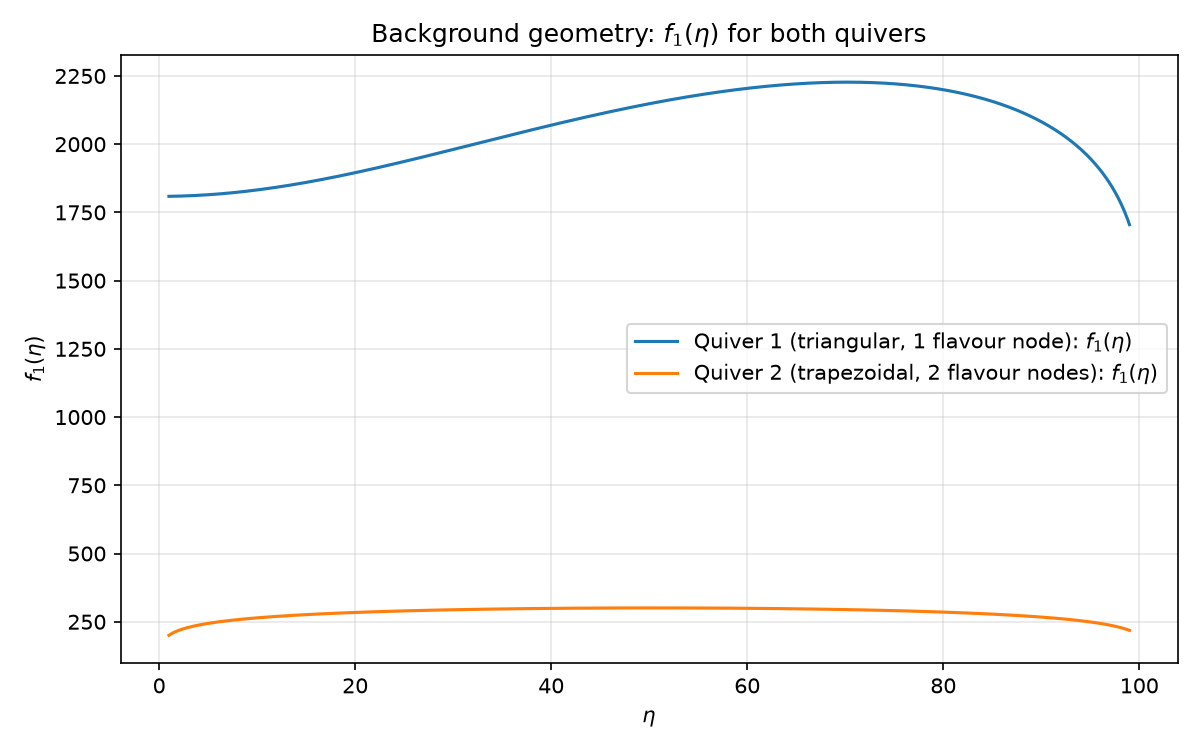
\includegraphics[width=0.75\linewidth]{../quiver_comparison/figures/01_geometry_f1_comparison.png}}
{\fbox{\parbox{0.7\linewidth}{\centering Figure to be inserted.}}}
\caption{The warp factor $f_1(\eta)$ for Quiver 1 (triangular rank, single flavour node) and Quiver 2 (trapezoidal rank, two flavour nodes), for the parameters of \cref{sec:quivers} ($N=1$, $P=100$). Quiver 1 is single-humped and roughly an order of magnitude larger in $f_1$ over the interior; Quiver 2 is flatter and more symmetric, reflecting its two flavour nodes. This difference in shape is the geometric origin of the numerical-window effect discussed below.}
\label{fig:quiver-f1-comparison}
\end{figure}

\subsection{Numerical comparison}

For representative values
\begin{equation*}
J\in\{0,1,3\},
\end{equation*}
the numerical calculations give the following pattern:
\begin{align*}
P_\rho^{\rm naive}(0)
&\simeq
\frac{|J|}{\sqrt{f_3(\eta_0)}},
\\
\PrhoR(0)
&\to0
\qquad (t\to0),
\end{align*}
for both quivers.

The numerical values reported in the project were
\begin{table}[H]
\centering
\begin{tabular}{@{}llrr@{}}
\toprule
Quiver & $J$ & $|J|/\sqrt{f_3(\eta_0)}$ & reported short-time trend\\
\midrule
1 & $1$ & $0.0877$ & $\PrhoR(t)\propto t$\\
1 & $3$ & $0.2630$ & $\PrhoR(t)\propto t$\\
2 & $1$ & $0.2307$ & $\PrhoR(t)\propto t$\\
2 & $3$ & $0.6920$ & $\PrhoR(t)\propto t$\\
\bottomrule
\end{tabular}
\caption{Representative naive intercepts and reduced short-time behaviour for the two quiver geometries.}
\label{tab:quiver-representative}
\end{table}

\begin{figure}[H]
\centering
\IfFileExists{../quiver_comparison/figures/09_naive_minus_routhian_intercept.png}
{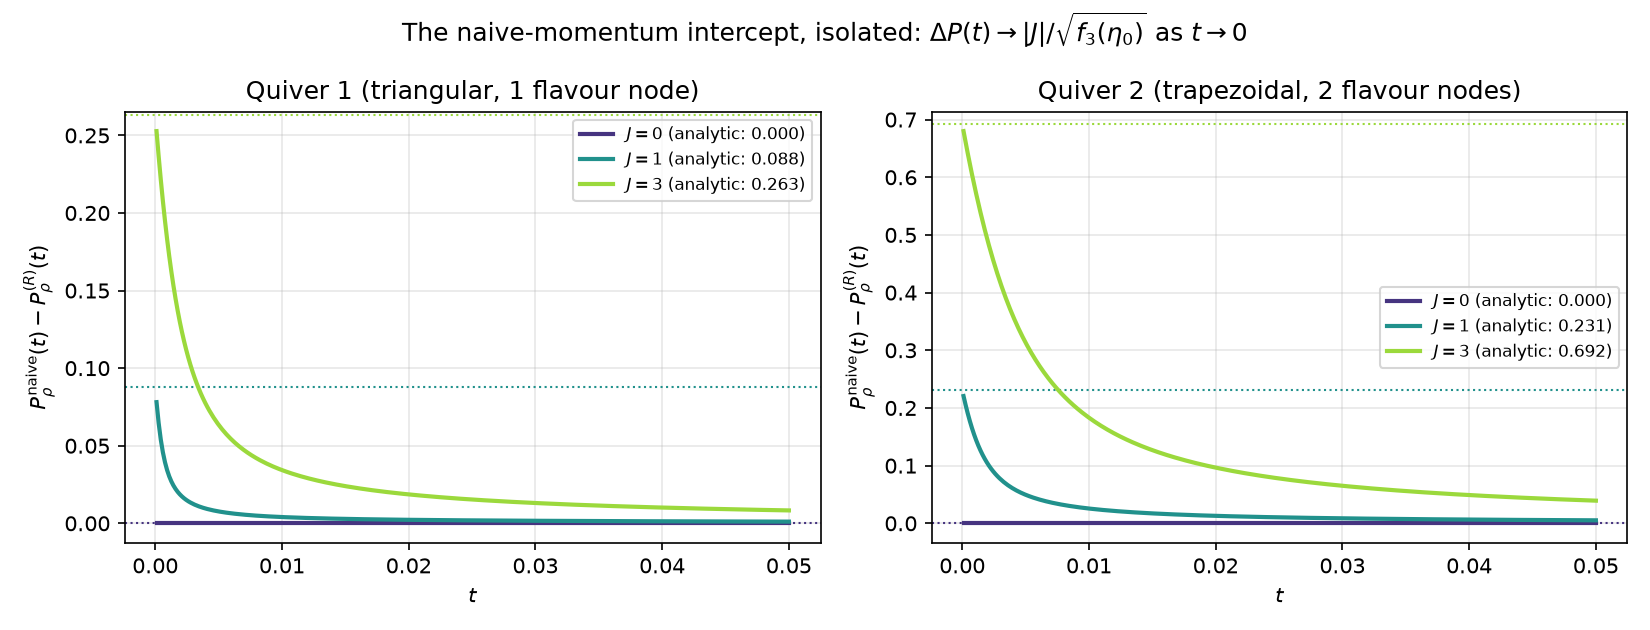
\includegraphics[width=0.95\linewidth]{../quiver_comparison/figures/09_naive_minus_routhian_intercept.png}}
{\fbox{\parbox{0.9\linewidth}{\centering Figure to be inserted from the project computation.}}}
\caption{The difference $P_\rho^{\mathrm{naive}}(t)-\PrhoR(t)$ as $t\to0^+$, for the two quivers and the three values of $J$ of \cref{tab:quiver-representative}. The numerical curves (solid) approach the analytic naive intercept $|J|/\sqrt{f_3(\eta_0)}$ (dotted horizontal lines, values as quoted in the legend), confirming that the entire discrepancy between the two prescriptions is accounted for by the intercept removed by the Routhian reduction.}
\label{fig:quiver-intercept}
\end{figure}

A technical point is important when reading the numerical tables. Values quoted as ``at $t=0$'' in the raw computation were sometimes evaluated at the first sampled time $t=10^{-4}$. A value of order $10^{-2}$ for the reduced momentum at that point is therefore consistent with a slope of order $10^2$, and should not be interpreted as a non-zero intercept.

\subsection{Numerical-window effect}

The two quivers also display a useful geometry-dependent difference. For the common initial point $\eta_0=50$, the second quiver places the probe close to the maximum of its relevant warp factor, whereas the first quiver places it farther from equilibrium. Consequently, higher-order terms in
\begin{equation*}
\PrhoR(t)=A_{\mathrm{6d}}t+B t^3+\cdots
\end{equation*}
become numerically visible earlier in the first quiver.

This explains the reported few-percent discrepancy between a finite-window slope estimate and the analytic $A_{\mathrm{6d}}$ for Quiver 1. The correct statement is therefore that the strict short-time coefficient is analytic, while a finite-time fit can be contaminated by the cubic correction. This distinction is important in order not to interpret a numerical fitting effect as a failure of the fixed-charge construction.

\subsection{Parameter scan}

The project also scanned the number of nodes
\begin{equation*}
P\in\{5,20,50,100,200\},
\end{equation*}
with $N=1$ and with the probe initially placed near the centre of the quiver interval. Across the tested family, the non-zero naive charge contribution and the vanishing fixed-charge intercept persisted, and the numerically extracted slope of $\PrhoR(t)$ tracks the analytic $A_{\mathrm{6d}}$ of \eqref{eq:6d-linear} at every value of $P$ tested, including the finite-window contamination for Quiver 1 discussed above (\cref{fig:quiver-P-scan}).

\begin{figure}[H]
\centering
\IfFileExists{../quiver_comparison/figures/10_scan_vs_P.png}
{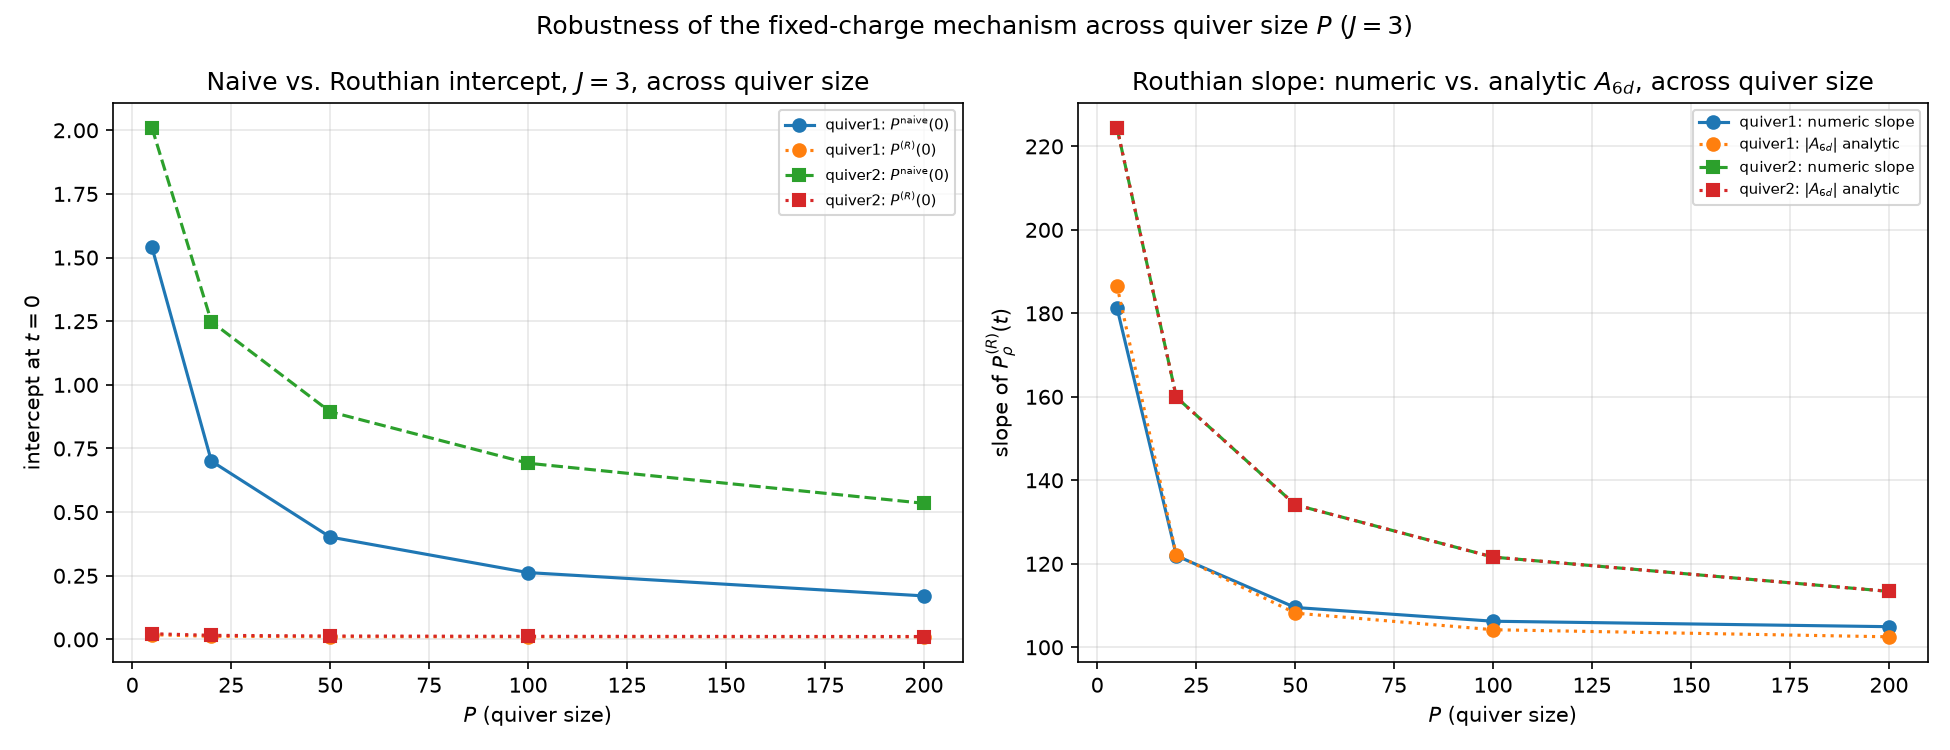
\includegraphics[width=0.95\linewidth]{../quiver_comparison/figures/10_scan_vs_P.png}}
{\fbox{\parbox{0.9\linewidth}{\centering Figure to be inserted from the project computation.}}}
\caption{Robustness of the fixed-charge mechanism across quiver size $P\in\{5,20,50,100,200\}$, at fixed $J=3$. \emph{Left:} the naive intercept $P_\rho^{\mathrm{naive}}(0)$ decreases with $P$ but remains strictly positive, while $\PrhoR(0)\approx0$ throughout. \emph{Right:} the numerically extracted slope of $\PrhoR(t)$ against the analytic $|A_{\mathrm{6d}}|$; the visible gap at small $P$ for Quiver 1 is the finite-window cubic contamination described in the text, not a failure of the short-time coefficient.}
\label{fig:quiver-P-scan}
\end{figure}

The calculation also found the scaling
\begin{equation}
f_i(\eta;N)
=
\sqrt N\,f_i(\eta;1),
\qquad i=1,2,3,
\label{eq:N-scaling}
\end{equation}
to full numerical precision. This is in fact an exact algebraic consequence of the construction of \cref{sec:6d}, not merely an empirical pattern. Both $\alpha''(\eta)=-81\pi^2NR(\eta)$ and the linear boundary conditions fixing $\alpha(\eta)$ are homogeneous of degree one in $N$, so $\alpha(\eta;N)=N\,\alpha(\eta;1)$, $\alpha'(\eta;N)=N\,\alpha'(\eta;1)$, and $\alpha''(\eta;N)=N\,\alpha''(\eta;1)$ identically. Under this rescaling, the combination $-\alpha/\alpha''$ appearing in $f_1,f_2,f_3$ is invariant, while $(\alpha')^2-2\alpha\alpha''$ scales as $N^2$; the dilaton factor $e^{\Phi}\propto(-\alpha/\alpha'')^{3/4}/\sqrt{(\alpha')^2-2\alpha\alpha''}$ therefore scales as $N^{-1}$, so $e^{-\Phi/2}\propto\sqrt N$. Since $f_1,f_2\propto e^{-\Phi/2}(-\alpha/\alpha'')^{\pm1/2}$ and $f_3\propto e^{-\Phi/2}\sqrt{-\alpha''/\alpha}\,\alpha^2/\big[(\alpha')^2-2\alpha\alpha''\big]$ carry no further net $N$-dependence beyond this dilaton factor, all three functions inherit the overall $\sqrt N$ -- exactly \eqref{eq:N-scaling}. This suggests that $P$, rather than $N$, is the more useful shape parameter for comparing quiver families in this setup.

The scan should nevertheless be interpreted as evidence over a finite parameter range rather than as a proof for arbitrary quiver data.

% ============================================================
\section{Quadratic black-string-chain background}
\label{sec:blackstring}
% ============================================================

\subsection{Motivation}

The final background considered in the project is structurally different from the 6d SCFT geometries above. Couzens et al.\ constructed $\mathcal N=(0,4)$ black-string chains in Type IIA supergravity from D2--D4--D6--NS5 intersections with fractional D4-branes \cite{Couzens:2021tnq}. Their near-horizon solutions contain an $\mathrm{AdS}_3$ factor, an $S^2$, a Calabi--Yau two-fold and an interval. The fractional-brane contribution allows a quadratic profile for one of the functions controlling the geometry.

The near-horizon Einstein-frame metric can be written as
\begin{equation*}
\mathrm d s_E^2
=
\frac1{\sqrt{h_4h_8}}
\left(
\mathrm d s_{\mathrm{AdS}_3}^2+\frac14\mathrm d s_{S^2}^2
\right)
+
\sqrt{\frac{h_4}{h_8}}\mathrm d s_{\mathrm{CY}_2}^2
+
\sqrt{h_4h_8}\mathrm d z^2,
\end{equation*}
with
\begin{equation*}
e^{-\Phi}=h_4^{1/4}h_8^{5/4}.
\end{equation*}
In the simplest flux sector,
\begin{equation*}
h_8=\gamma,
\qquad
\partial_z^2h_4=-\gamma,
\end{equation*}
so locally
\begin{equation*}
h_4(z)
=
\alpha+\beta z-\frac{\gamma}{2}z^2.
\end{equation*}

\subsection{Restricted probe dynamics}

Following the project setup, the probe is allowed to move in $(r,z,\varphi)$ while the Calabi--Yau directions and the transverse AdS coordinate are frozen, and the $S^2$ polar angle is fixed at the equator. The induced Lagrangian takes the generic form
\begin{equation}
\mathcal L
=
-m\sqrt{
F_1(z)(e^{-\lambda r}-\dot r^2)
-F_2(z)\dot z^2
-F_3(z)\dot\varphi^2
},
\label{eq:blackstring-lagrangian}
\end{equation}
where, for the simplest sector,
\begin{equation}
\boxed{
F_1(z)=\gamma^{1/8}h_4(z)^{-3/8},
\qquad
F_3(z)=\frac14F_1(z),
\qquad
F_2(z)=\gamma^{9/8}h_4(z)^{5/8}.
}
\label{eq:blackstring-Fi}
\end{equation}

The fixed-charge Routhian is again
\begin{equation*}
R
=
-\meff(z)
\sqrt{
F_1(z)(e^{-\lambda r}-\dot r^2)-F_2(z)\dot z^2
},
\qquad
\meff(z)
=
\sqrt{
m^2+\frac{J^2}{F_3(z)}
}.
\end{equation*}

\begin{figure}[H]
\centering
\IfFileExists{../blackstring_quiver/figures/02_naive_vs_routhian.png}
{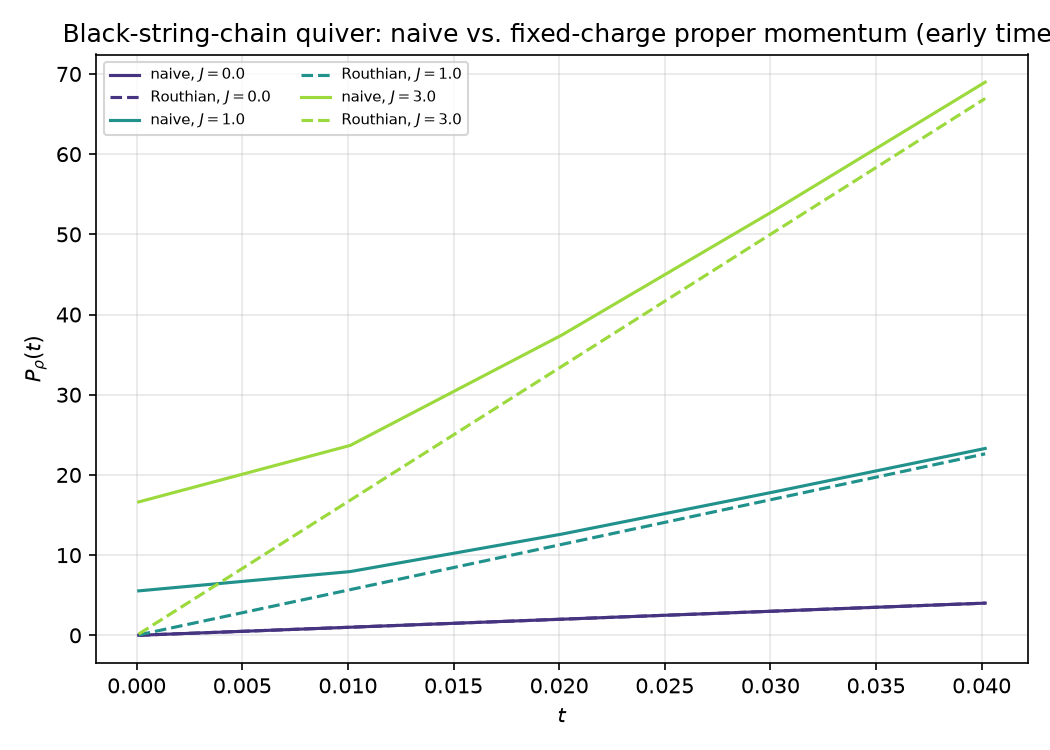
\includegraphics[width=0.72\linewidth]{../blackstring_quiver/figures/02_naive_vs_routhian.png}}
{\fbox{\parbox{0.68\linewidth}{\centering Figure to be inserted.}}}
\caption{Naive versus fixed-charge composite proper momentum $P_\rho(t)$ at early times, for the black-string-chain background and $J\in\{0,1,3\}$. As in the point-particle and quiver cases, the naive prescription (solid) sits at a nonzero value already at the earliest plotted times, while the Routhian-reduced prescription (dashed) starts from zero.}
\label{fig:bs-naive-vs-routhian}
\end{figure}

\subsection{Exact radial relation}

The radial solution can be written
\begin{equation}
\lambda r(t)
=
\log
\left(
e^{\lambda r_{\rm UV}}
+
\frac{\lambda^2t^2}{4}
\right),
\label{eq:bs-r}
\end{equation}
with
\begin{equation*}
\dot r(t)
=
\frac{\lambda t/2}
{
e^{\lambda r_{\rm UV}}+\lambda^2t^2/4
}.
\end{equation*}
The same conserved-energy argument as above then gives
\begin{equation*}
\boxed{
P_r^{(R)}(t)
=
\frac{\lambda H}{2}\,t,
}
\end{equation*}
under the assumptions of the reduced background. For $\lambda=2$, this reduces to
\begin{equation*}
P_r^{(R)}(t)=Ht.
\end{equation*}

The exact radial linearity is independent of the detailed form of $h_4(z)$. The geometry dependence enters the $z$-sector and the composite reduced proper momentum.

\subsection{UV rescaling of the quiver trajectory}

A useful additional observation is that the dependence on the UV cutoff can be isolated by defining
\begin{equation*}
x
=
\frac{\lambda}{2}
e^{-\lambda r_{\rm UV}/2}t.
\end{equation*}
Using \eqref{eq:bs-r}, one finds
\begin{equation*}
e^{-\lambda r}-\dot r^2
=
\frac{
e^{-\lambda r_{\rm UV}}
}{
(1+x^2)^2
},
\end{equation*}
and
\begin{equation*}
\dot z
=
\frac{\lambda}{2}
e^{-\lambda r_{\rm UV}/2}
\frac{\mathrm d z}{\mathrm d x}.
\end{equation*}
Hence the reduced action can be written
\begin{equation}
S
=
-\frac2\lambda
\int
\meff(z)
\sqrt{
\frac{F_1(z)}{(1+x^2)^2}
-
\frac{\lambda^2}{4}
F_2(z)
\left(\frac{\mathrm d z}{\mathrm d x}\right)^2
}
\,\mathrm d x.
\label{eq:scaled-action}
\end{equation}
All explicit $r_{\rm UV}$-dependence has disappeared.

\begin{proposition}[UV rescaling property]
\label{prop:uv-rescaling}
For the restricted class of black-string-chain probe problems described by \eqref{eq:blackstring-lagrangian}, if the initial quiver coordinate and its initial derivative with respect to $x$ are held fixed, then the quiver trajectory $z(x)$ is independent of $r_{\rm UV}$. Changing $r_{\rm UV}$ changes only the map between physical time $t$ and the scaled time $x$.
\end{proposition}

\begin{proof}
Equation \eqref{eq:scaled-action} contains no explicit $r_{\rm UV}$. The initial data
\begin{equation*}
z(0)=z_0,
\qquad
z'(0)=0
\end{equation*}
are also independent of $r_{\rm UV}$. Therefore the Euler--Lagrange initial-value problem in the variable $x$ is the same for every $r_{\rm UV}$ for which the solution exists uniquely.
\end{proof}

This result means that making the UV cutoff deeper cannot turn a non-crossing trajectory into a crossing trajectory in this reduced system: it only changes the physical time at which a given value of the universal scaled trajectory is reached.

\subsection{Multi-well structure}

For the benchmark choice used in the project, the quadratic $h_4(z)$ develops several local maxima separated by interior minima at the kinks. This produces a multi-well landscape that is qualitatively different from the single-hump $f_1(\eta)$ profiles encountered for the two linear-quiver examples.

The project calculations used the reference benchmark
\begin{equation*}
P=6,\qquad
\gamma=32,\qquad
(\beta_0,\ldots,\beta_5)=(22,21,19,17,15,15),
\end{equation*}
with $\beta_6$ fixed by the closing condition. In the numerical profile, the local maxima lie within the individual segments, while the interior kinks act as barriers.

\begin{figure}[H]
\centering
\IfFileExists{../blackstring_quiver/figures/01_h4_profile.png}
{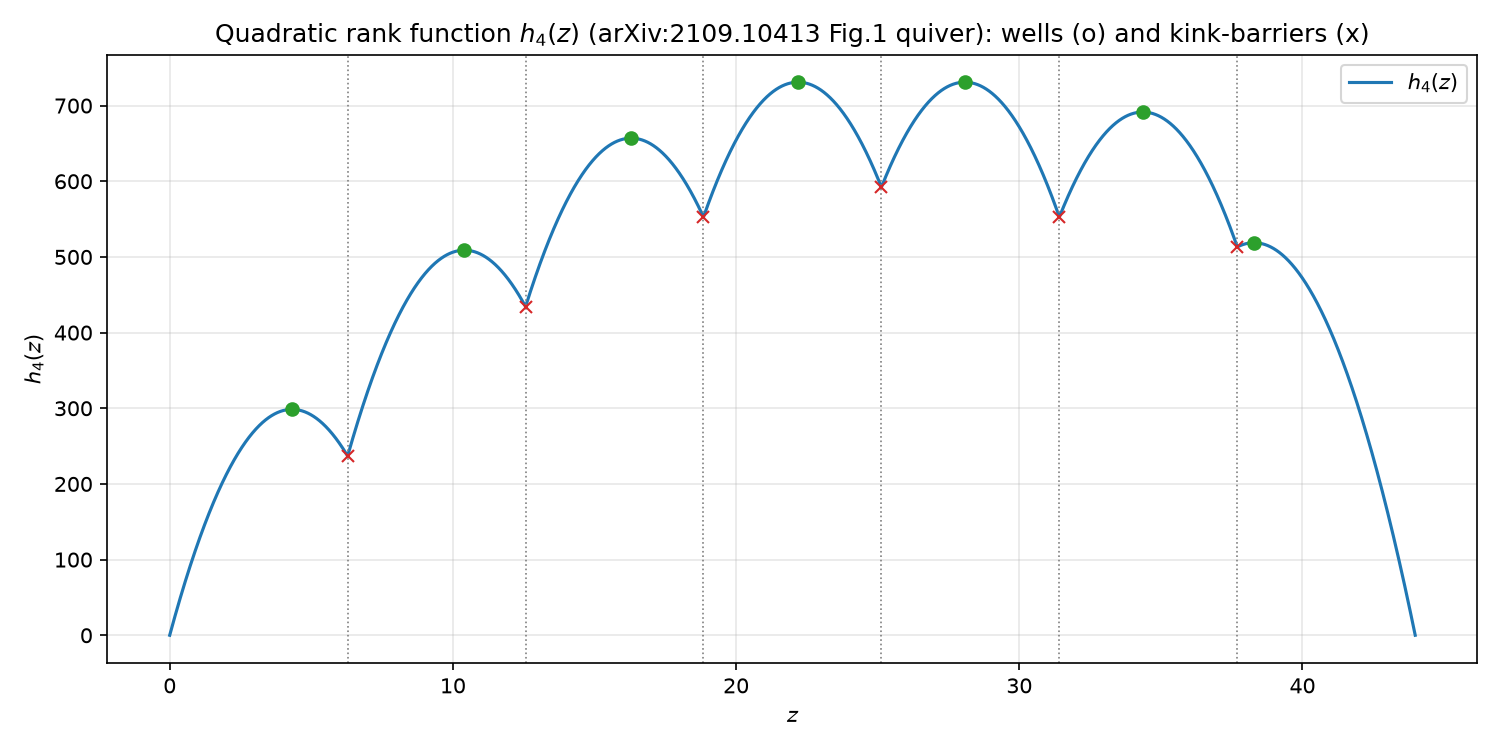
\includegraphics[width=0.78\linewidth]{../blackstring_quiver/figures/01_h4_profile.png}}
{\fbox{\parbox{0.72\linewidth}{\centering Quadratic $h_4(z)$ profile to be inserted from the project computation.}}}
\caption{Representative quadratic black-string-chain profile. The quadratic term produces a multi-well structure separated by kink locations.}
\label{fig:blackstring-h4}
\end{figure}

\subsection{Numerical observations on confinement}

The project numerically investigated whether a probe could cross from one local well into a neighbouring well. For the reference benchmark and initial conditions tested, the displacement in $z$ was extremely small compared with the distance to the nearest barrier.

A special feature of this background is that $F_1(z)/F_3(z)=4$ identically, independent of $z$ (this follows directly from \eqref{eq:blackstring-Fi}). Consequently the equilibrium position selected by the $J=0$ dynamics, $z^\ast=\operatorname{argmax}F_1(z)=\operatorname{argmax}h_4(z)$, does not shift with $J$: charging the probe changes the amplitude and time-scale of the residual oscillation around $z^\ast$ but not the equilibrium itself, exactly as illustrated in \cref{fig:bs-J-independence}.

For example, in the benchmark well considered in the project, the reported displacement remained of order
\begin{equation*}
\Delta z\sim 10^{-7}
\end{equation*}
while the nearest barrier was separated by a distance of order unity. A smaller benchmark with the minimal allowed even $\gamma$ produced a larger displacement, but it remained far below the barrier scale.

\begin{figure}[H]
\centering
\IfFileExists{../blackstring_quiver/figures/03_J_independent_equilibrium.png}
{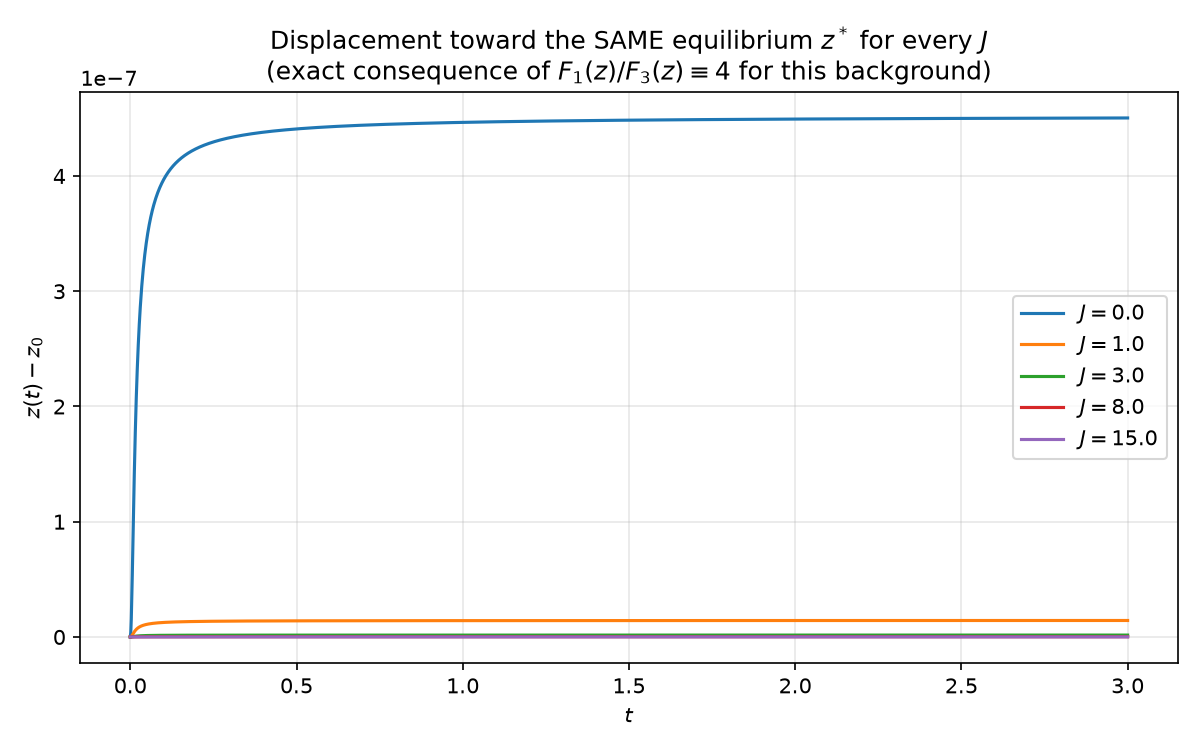
\includegraphics[width=0.72\linewidth]{../blackstring_quiver/figures/03_J_independent_equilibrium.png}}
{\fbox{\parbox{0.68\linewidth}{\centering Figure to be inserted.}}}
\caption{Displacement $z(t)-z_0$ from the well maximum, released one unit off-centre, for $J\in\{0,1,3,8,15\}$. All curves saturate at the same order-$10^{-7}$ displacement scale and approach the same equilibrium, the exact consequence of $F_1(z)/F_3(z)\equiv4$ noted in the text; increasing $J$ suppresses rather than shifts the residual motion.}
\label{fig:bs-J-independence}
\end{figure}

These calculations support the following qualified statement:

\begin{observation}
For the black-string-chain examples and parameter choices explicitly explored in the project, no transition between neighbouring wells was observed. The UV-rescaling property shows that this conclusion is not changed merely by varying the UV cutoff within the same reduced trajectory family.
\end{observation}

This is intentionally weaker than a theorem that no allowed black-string-chain quiver can ever exhibit hopping. Such a universal statement would require an analytic bound on the maximum attainable $z$-displacement over the full allowed parameter space, which has not been established here.

% ============================================================
\section{Universal mechanism and geometry-dependent data}
\label{sec:universal}
% ============================================================

The calculations naturally split into two categories.

\subsection{Structural statements}

The following features arise from the fixed-charge reduction itself:

\begin{enumerate}[leftmargin=2em]
\item A cyclic coordinate $\varphi$ gives a conserved Noether charge $J$.
\item The unreduced proper momentum contains a charge-dependent contribution that need not vanish at a radial turning point.
\item Fixing $J$ and eliminating $\varphi$ with a Routhian retains the charge through an effective mass or potential.
\item The reduced momenta associated with the non-cyclic coordinates vanish when those velocities vanish.
\item A smooth turning-point trajectory therefore produces reduced momentum proportional to $t$ at short times.
\item Identifying the complexity growth rate with the magnitude of the reduced proper momentum is consequently compatible with $\Ck(t)\sim t^2$.
\end{enumerate}

These are the most robust conclusions because they depend primarily on the cyclic structure of the probe Lagrangian rather than on detailed properties of a specific background. The same basic mechanism is also the central message of the recent fixed-charge analysis of holographic spread complexity \cite{Chatzis:2026ekd}.

\subsection{Geometry-dependent statements}

The following quantities remain sensitive to the background: the short-time coefficient $A(J,m,r_0)$, the effective mass $\meff$, equilibrium positions, higher-order coefficients, and global trajectories. In the six-dimensional SCFT examples, the detailed quiver dependence enters through $f_1,f_2,f_3$. In the black-string-chain background, the quadratic $h_4$ profile changes the quiver-direction landscape without changing the algebraic structure of the Routh reduction.

\subsection{What the result does not prove}

The present calculations do not by themselves establish:
\begin{itemize}[leftmargin=2em]
\item a first-principles derivation of the full quantum gravity dictionary
\begin{equation*}
\dot{\Ck}=\lambda|\PrhoR|
\end{equation*}
for arbitrary charged states;
\item a universal value of the normalization $\lambda$;
\item a universal absence of well-to-well hopping in all allowed black-string-chain backgrounds;
\item a complete field-theoretic construction of the corresponding fixed-$J$ Krylov basis.
\end{itemize}

The analytic result is a \emph{consistency and reduction statement}; the numerical calculations are validations of that statement in selected geometries.

% ============================================================
\section{Numerical methodology}
\label{sec:numerics}
% ============================================================

The numerical checks in the project follow the same overall procedure.

\subsection{Geodesic integration}

For each geometry, the initial data specify the starting point and the turning-point condition. The conserved charge $J$ is fixed, while the remaining equations are integrated either as a second-order Euler--Lagrange system or in a first-order form when an energy integral is available.

An adaptive Runge--Kutta method such as RK45 is sufficient for the smooth trajectories considered here. At each time step one evaluates the original and reduced momenta and compares:
\begin{equation*}
P_{\mathrm{naive}}(t),
\qquad
\PrhoR(t),
\qquad
\frac{\PrhoR(t)}{t},
\qquad
\frac{\Ck(t)}{t^2}
\end{equation*}
in the short-time regime.

\subsection{Diagnostics}

The most informative diagnostics are:

\paragraph{Intercept test.}
The naive observable should approach
\begin{equation*}
\frac{|J|}{\sqrt{h(r_0)}}
\quad\text{or}\quad
\frac{|J|}{\sqrt{f_3(\eta_0)}},
\end{equation*}
depending on the background, whereas the reduced observable should approach zero.

\paragraph{Slope test.}
The ratio
\begin{equation*}
\frac{\PrhoR(t)}{t}
\end{equation*}
should approach a finite constant as $t\to0^+$. This constant can be compared with the analytic coefficient.

\paragraph{Quadratic-complexity test.}
If the holographic relation is integrated as
\begin{equation*}
\Ck(t)
=
\int_0^t
\lambda|\PrhoR(t')|\,\mathrm d t',
\end{equation*}
then
\begin{equation*}
\frac{\Ck(t)}{t^2}
\end{equation*}
should approach a constant.

\paragraph{Resolution test.}
Since the central statement concerns the strict limit $t\to0$, slope fits should be repeated over progressively smaller time windows. A discrepancy that decreases with the window size is evidence for higher-order contamination rather than a failure of the analytic short-time coefficient.

\subsection{Interpretation of numerical precision}

Machine-level agreement of an algebraic identity after integrating an ODE is a useful code-consistency check, but it is not by itself a physical theorem. The report therefore distinguishes exact algebraic identities, analytic short-time limits, and finite-resolution numerical comparisons.

% ============================================================
\section{Discussion}
\label{sec:discussion}
% ============================================================

The main conceptual lesson is that one must compare the \emph{same dynamical sector} on both sides of the holographic dictionary. Krylov complexity can be studied in sectors of fixed global quantum numbers. On the bulk side, the corresponding Noether charge should therefore be held fixed before the momentum observable is defined.

The Routhian implements precisely this reduction. The cyclic coordinate disappears from the reduced configuration space, while its energy contribution becomes part of an effective mass:
\begin{equation*}
m
\quad\longrightarrow\quad
\sqrt{m^2+\frac{J^2}{h}}
\end{equation*}
for the simple point-particle model, or
\begin{equation*}
m
\quad\longrightarrow\quad
\sqrt{m^2+\frac{J^2}{f_3(\eta)}}
\end{equation*}
for the six-dimensional quiver backgrounds.

This also clarifies the slogan used in the oral presentation:
\begin{quote}
\emph{Fix the conserved charge before constructing the proper momentum.}
\end{quote}
It should not be interpreted as a new physical time-ordering operation. It is a statement about the order of reduction: first restrict to the fixed-$J$ sector and eliminate the cyclic degree of freedom, then construct the proper momentum of the reduced system.

The distinction between the radial and composite reduced momenta is also important. In the $\mathrm{AdS}_7$ examples the radial component obeys an exact linear identity under the assumptions of the setup, whereas the composite $(r,\eta)$ momentum retains geometry-dependent information. Thus the geometry may affect subleading and transverse spreading without changing the leading radial structure.

% ============================================================
\section{Conclusions and outlook}
\label{sec:conclusions}
% ============================================================

This report has studied the short-time consistency of holographic Krylov complexity for probes carrying conserved charges.

The quantum side gives a universal baseline:
\begin{equation*}
\Ck(t)=b_1^2t^2+\mathcal O(t^4),
\qquad
\dot{\Ck}(0)=0.
\end{equation*}
A naive bulk momentum that includes a non-zero cyclic contribution at a radial turning point violates this condition.

The fixed-charge Routhian resolves the mismatch. At fixed $J$, the cyclic coordinate is removed through a partial Legendre transform and its effect survives through an effective mass or potential. The reduced proper momentum then vanishes for a probe released from rest and grows linearly at short times.

The mechanism was developed analytically for a general charged point particle and made explicit in global $\mathrm{AdS}_3$, where a closed-form short-time coefficient was obtained. The same construction was then applied to two top-down six-dimensional SCFT quivers. Finally, the reduction was extended to a structurally different quadratic black-string-chain background. The numerical results support the persistence of the fixed-charge mechanism across these examples, while also revealing that detailed coefficients, equilibration and quiver-direction motion remain geometry dependent.

Several questions remain open. The most immediate is whether the same fixed-charge structure survives for genuinely extended probes, in particular D-brane probes with worldvolume dynamics and additional conserved charges; charged, composite and extended probes of this kind have begun to be analysed directly in \cite{Nastase:2026lhz}, and the fixed-charge Routhian construction used here is a natural point of contact with that programme. A second direction is to identify the precise field-theoretic counterpart of the reduced bulk observable, for example through a symmetry-resolved Krylov construction. A third is to derive analytic bounds on quiver-direction displacement in the black-string-chain backgrounds and determine whether barrier crossing can occur in any allowed parameter regime.

The central conclusion can therefore be summarized as
\begin{equation*}
\boxed{
\begin{gathered}
\text{At fixed conserved charge, the reduced holographic momentum}\\
\text{has the correct short-time behaviour required by Krylov complexity.}
\end{gathered}}
\end{equation*}

% ============================================================
\appendix
\section{Detailed derivation of the point-particle Routhian}
\label{app:routhian-detail}
% ============================================================

Starting from
\begin{equation*}
L=-mD,
\qquad
D=
\sqrt{
f-g\dot r^2-h\dot\varphi^2
},
\end{equation*}
the charge constraint reads
\begin{equation*}
J=\frac{mh\dot\varphi}{D}.
\end{equation*}
Solving for $\dot\varphi$ gives
\begin{equation*}
D=\frac{mh\dot\varphi}{J},
\end{equation*}
and therefore
\begin{equation*}
\frac{m^2h^2\dot\varphi^2}{J^2}
=
f-g\dot r^2-h\dot\varphi^2.
\end{equation*}
Rearranging,
\begin{align*}
\dot\varphi^2
\left(
\frac{m^2h^2}{J^2}+h
\right)
&=
f-g\dot r^2,
\\
\dot\varphi^2
&=
\frac{
J^2(f-g\dot r^2)
}{
h(J^2+m^2h)
}.
\end{align*}
Choosing the sign consistent with $J$,
\begin{equation*}
\dot\varphi
=
\frac{
J\sqrt{f-g\dot r^2}
}{
\sqrt{h(J^2+m^2h)}
}.
\end{equation*}
The Routhian in the convention \eqref{eq:our-routhian-convention} is
\begin{align*}
R
&=
-mD-J\dot\varphi
\\
&=
-\frac{m^2h+J^2}{J}\dot\varphi
\\
&=
-\frac{m^2h+J^2}{J}
\frac{
J\sqrt{f-g\dot r^2}
}{
\sqrt{h(J^2+m^2h)}
}
\\
&=
-\sqrt{
m^2+\frac{J^2}{h}
}
\sqrt{
f-g\dot r^2
}.
\end{align*}
This proves \eqref{eq:reduced-routhian}.

% ============================================================
\section{General short-time coefficient}
\label{app:A}
% ============================================================

For
\begin{equation*}
R(r,\dot r;J)
=
-\meff(r)\sqrt{f(r)-g(r)\dot r^2},
\end{equation*}
with
\begin{equation*}
\meff(r)=\sqrt{m^2+\frac{J^2}{h(r)}},
\end{equation*}
the Euler--Lagrange equation is
\begin{equation*}
\frac{\mathrm d}{\mathrm d t}\PrR
=
\frac{\partial R}{\partial r}.
\end{equation*}
At a turning point $\dot r(0)=0$,
\begin{equation*}
\PrR(0)=0.
\end{equation*}
Since
\begin{equation*}
R(r,0;J)
=
-\meff(r)\sqrt{f(r)},
\end{equation*}
we have
\begin{equation*}
\left.\frac{\mathrm d\PrR}{\mathrm d t}\right|_{t=0}
=
-\meff'(r_0)\sqrt{f(r_0)}
-
\frac{\meff(r_0)f'(r_0)}
{2\sqrt{f(r_0)}}.
\end{equation*}
Thus
\begin{equation*}
\boxed{
A(J,m,r_0)
=
-\meff'(r_0)\sqrt{f(r_0)}
-
\frac{\meff(r_0)f'(r_0)}
{2\sqrt{f(r_0)}}.
}
\end{equation*}
Using
\begin{equation*}
\meff'(r)
=
-\frac{
J^2h'(r)
}{
2h(r)^2\meff(r)
},
\end{equation*}
this becomes
\begin{equation*}
A
=
\frac{
J^2h'(r_0)\sqrt{f(r_0)}
}{
2h(r_0)^2\meff(r_0)
}
-
\frac{
\meff(r_0)f'(r_0)
}{
2\sqrt{f(r_0)}
}.
\end{equation*}

For global $\mathrm{AdS}_3$ this reduces to \eqref{eq:ads3-alpha}.

% ============================================================
\section{Additional numerical checks and reproducibility}
\label{app:numerics}
% ============================================================

The project computations used separate scripts for:
\begin{itemize}[leftmargin=2em]
\item geometry construction;
\item Routhian reduction;
\item symbolic checks of the quiver-2 construction;
\item numerical geodesic integration;
\item parameter scans.
\end{itemize}

For the final MIORPA submission, these scripts should be kept together with the report so that every numerical figure can be regenerated from the stated parameters.

A particularly important reproducibility convention is to distinguish:
\begin{equation*}
P(0)
\end{equation*}
from
\begin{equation*}
P(t_{\min})
\end{equation*}
when $t_{\min}>0$ is the first sampled time. This avoids interpreting a finite-time value of a linearly vanishing momentum as a non-zero initial intercept.

% ============================================================
\bibliographystyle{JHEP}
\bibliography{Krylov}

\end{document}
